\section{Illustrations}
\subsection{Scrum}
\label{scrumillustrations}
% Scrum pictures
\begin{figure}[H]
  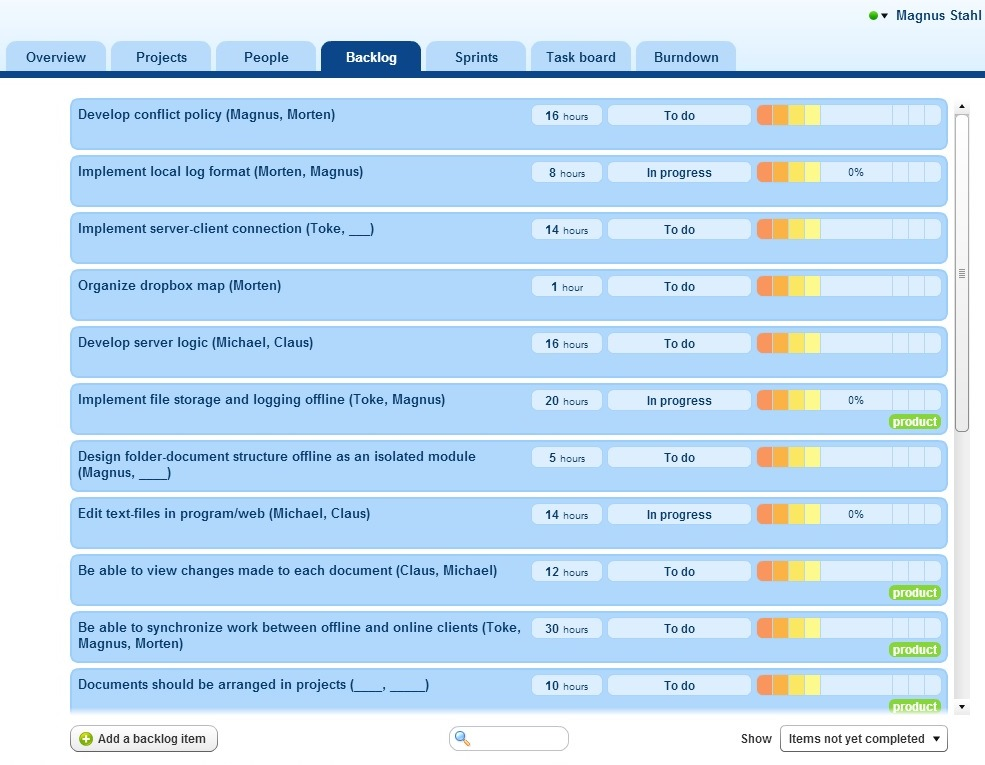
\includegraphics[width=\textwidth,natwidth=985,natheight=765]{illustrations/backlog1.jpeg}
  \caption{Backlog}
  \label{backlog1}
\end{figure}
\begin{figure}[H]
  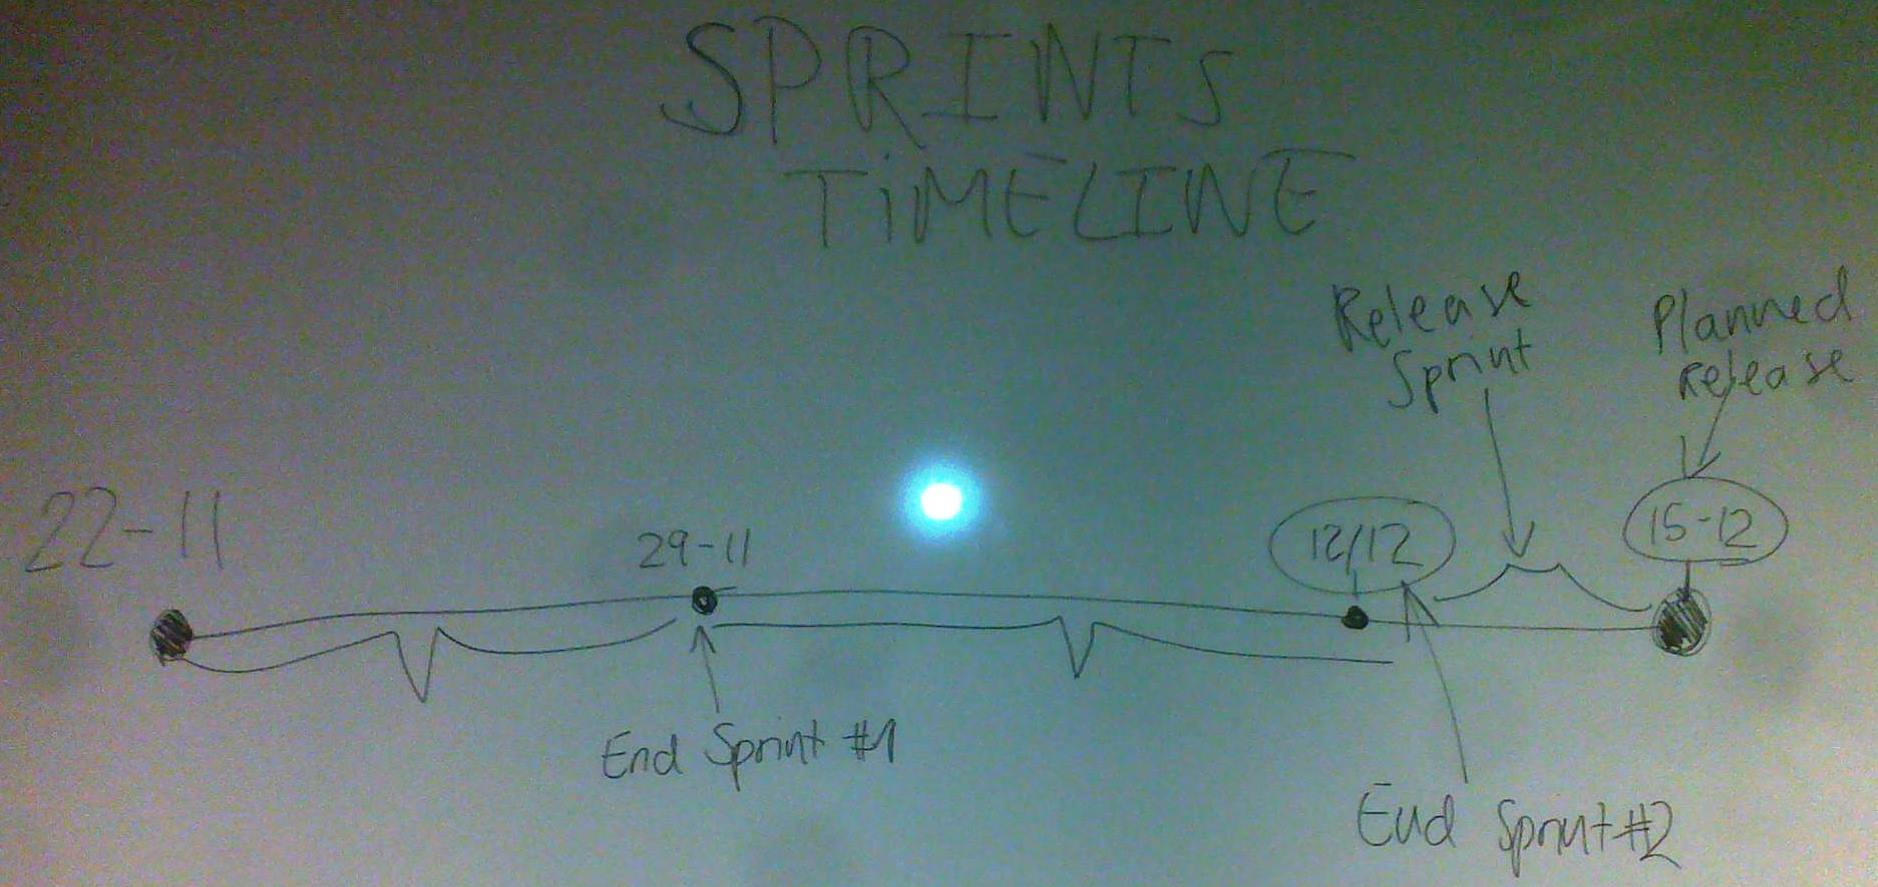
\includegraphics[width=\textwidth]{illustrations/04122012107.jpg}
  \caption{Sprint Timeline}
  \label{sprinttimeline}
\end{figure}
\begin{figure}[H]
  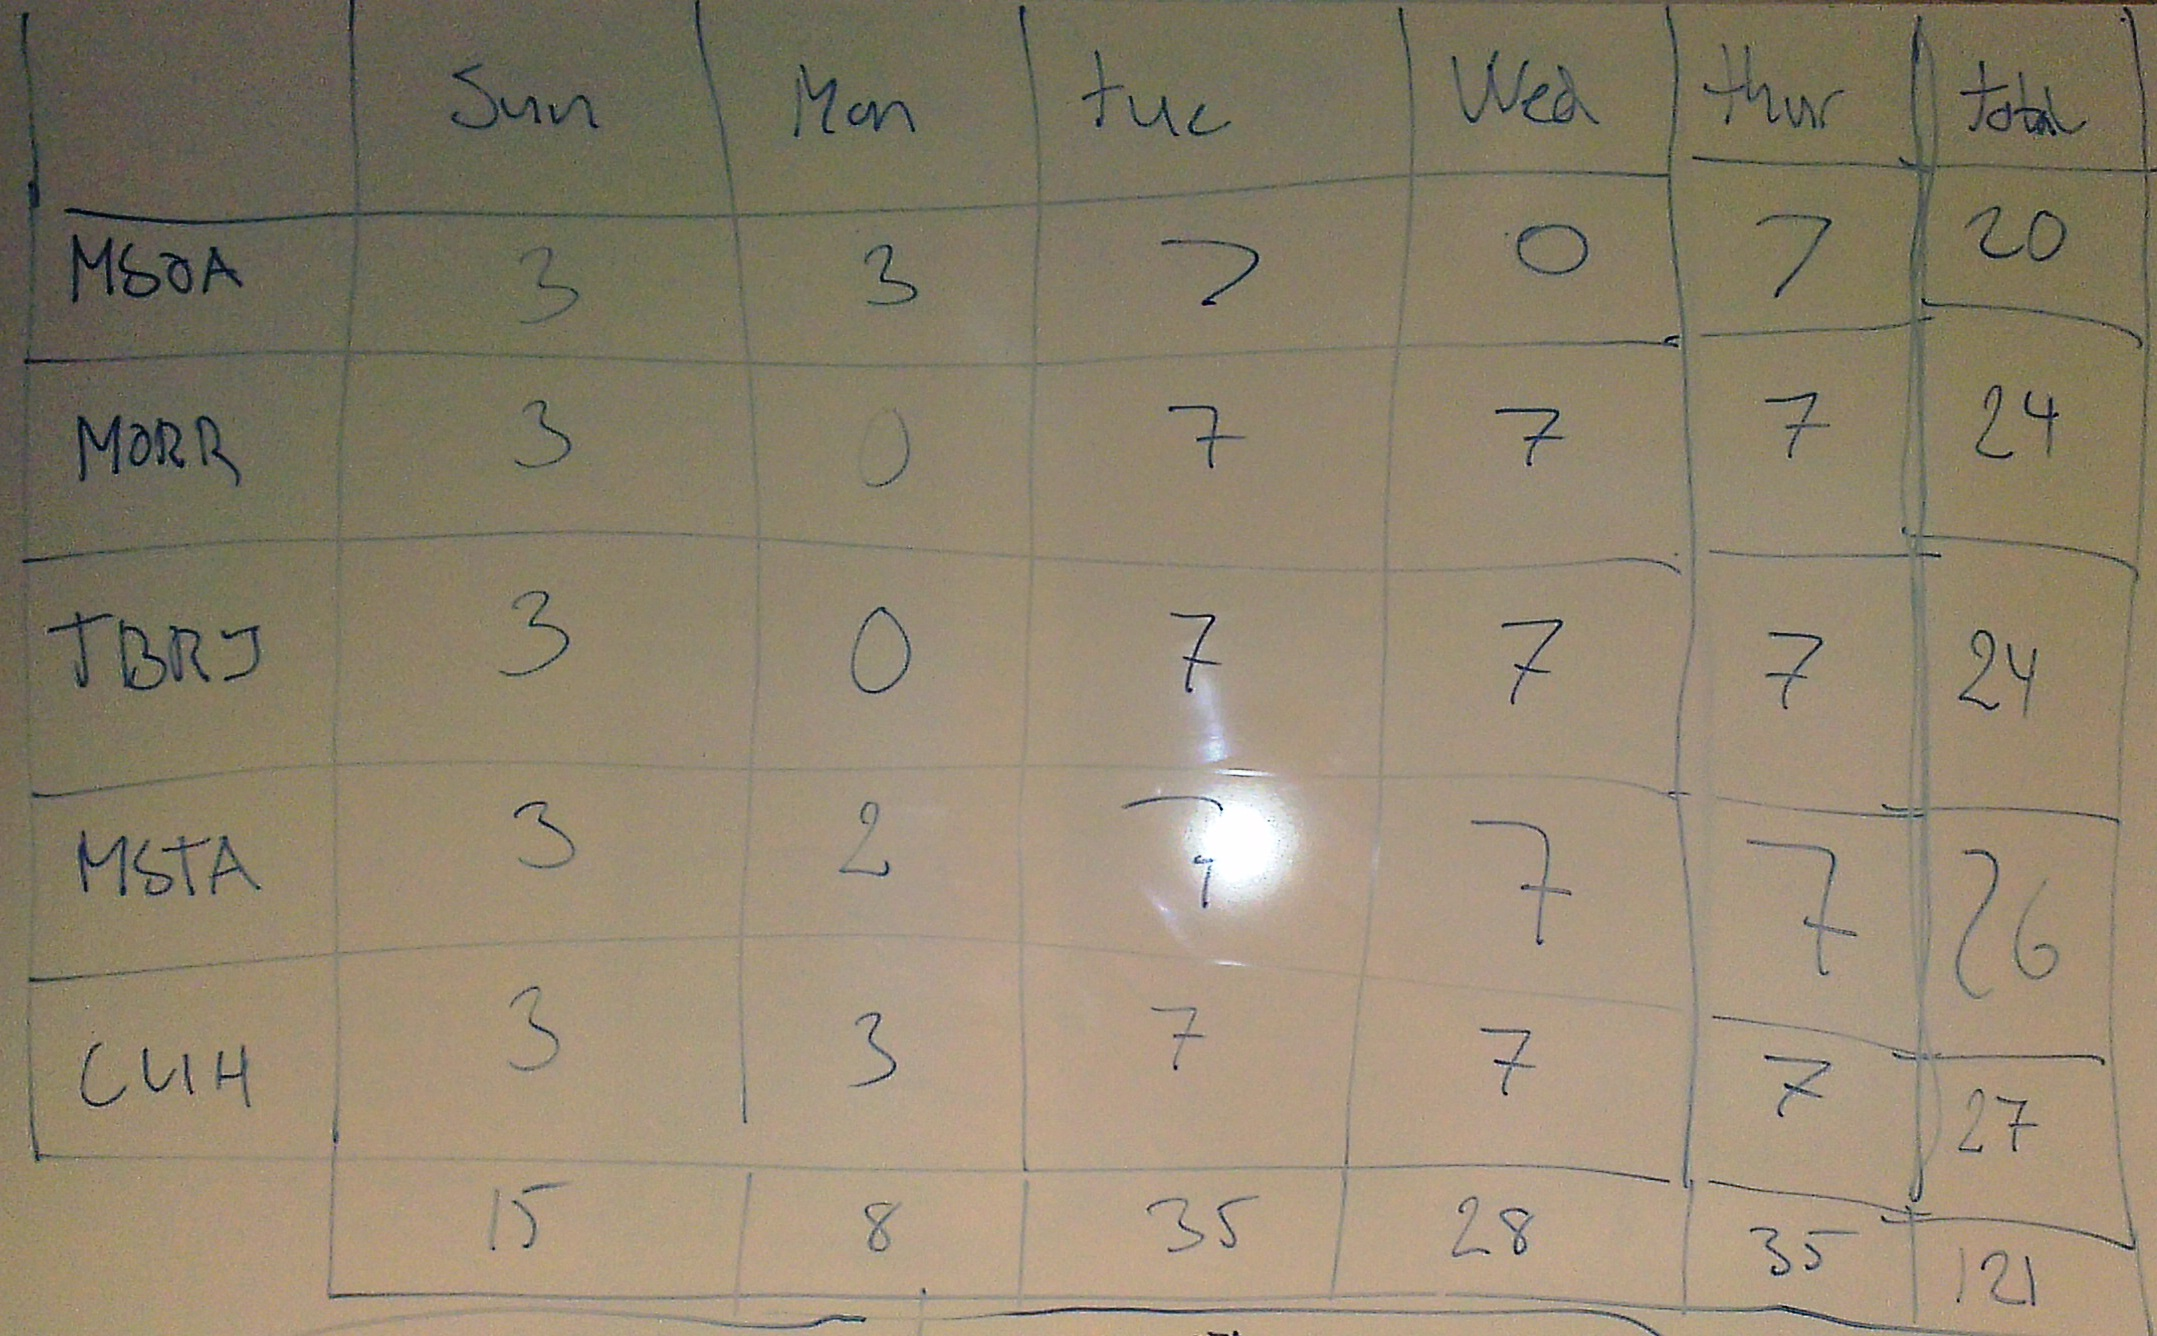
\includegraphics[width=\textwidth,natwidth=2157,natheight=1336]{illustrations/CapacityPlan.jpg}
  \caption{Capacity Plan}
  \label{capacityplan}
\end{figure}
\begin{figure}[H]
  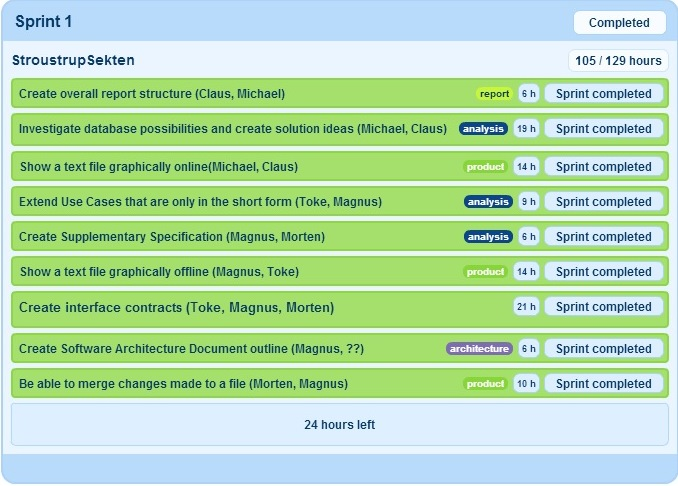
\includegraphics[width=\textwidth,natwidth=678,natheight=486]{illustrations/sprintbacklog1.jpeg}
  \caption{Sprint1 Backlog}
  \label{sprint1backlog}
\end{figure}
\subsection{Package Diagram}
\begin{figure}[H]
  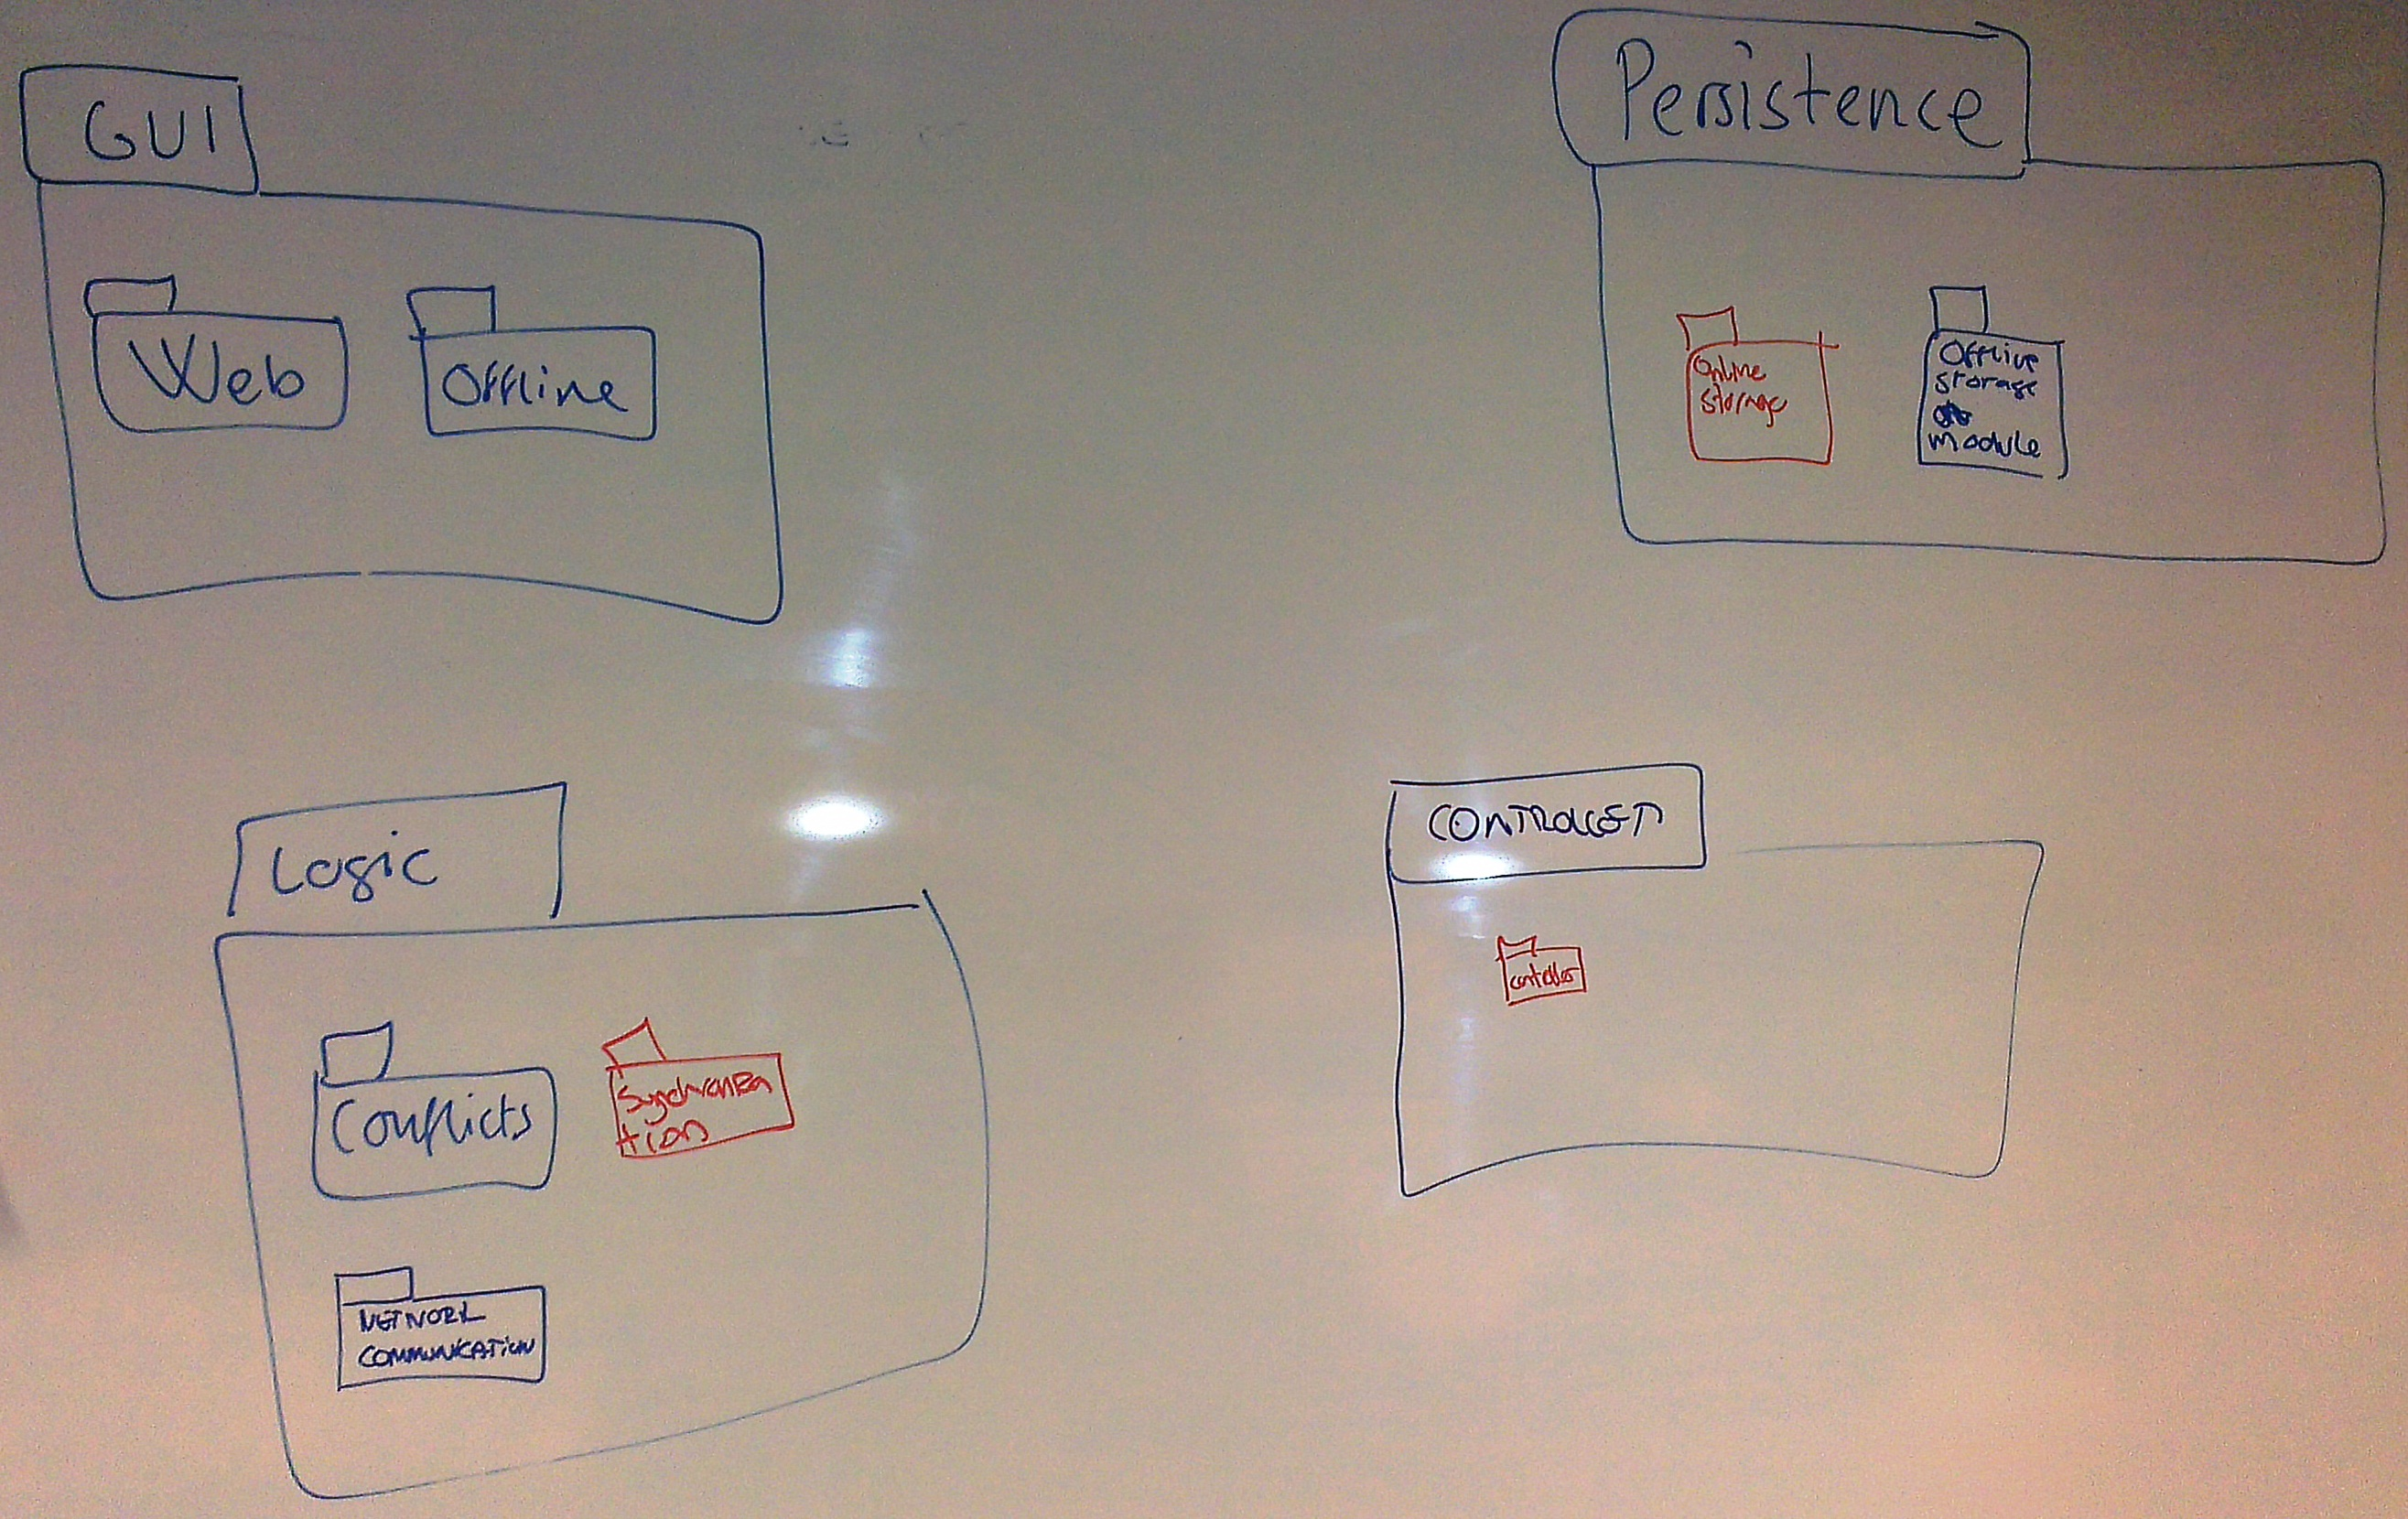
\includegraphics[width=\textwidth,natwidth=2631,natheight=1660]{illustrations/PackageDiagram.jpg}
  \caption{Package Diagram}
  \label{packagediagram}
\end{figure}
\subsection{Deployment Diagram}
\begin{figure}[H]
  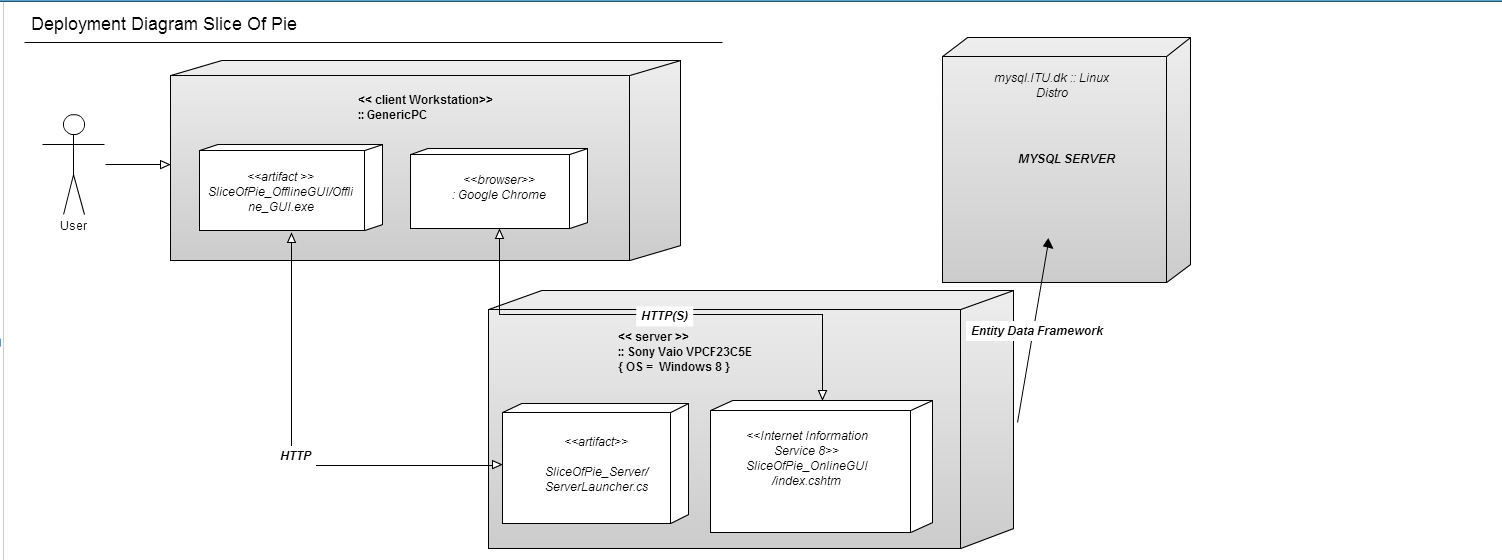
\includegraphics[width=\textwidth]{illustrations/deploymentDiagram.PNG}
  \caption{Deployment Diagram}
  \label{deploymentdiagram}
\end{figure}
\subsection{Class Diagrams}
\label{classdiagrams}
\begin{figure}[H]
  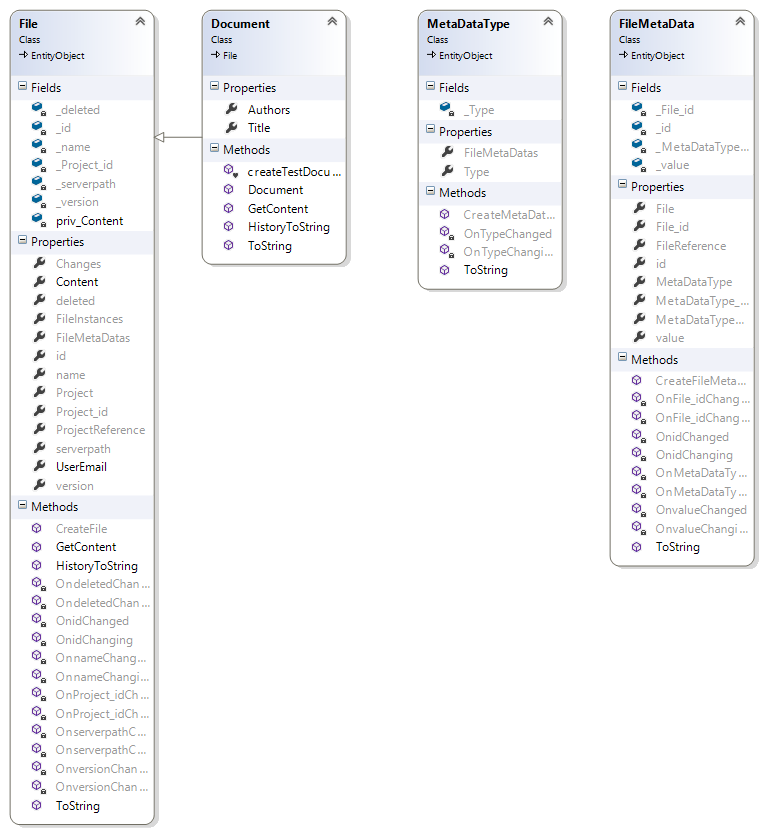
\includegraphics[width=\textwidth]{illustrations/classDiagrams/FileOverviewRep_CD.png}
  \caption{Class Diagram File Overview}
\end{figure}
\begin{figure}[H]
  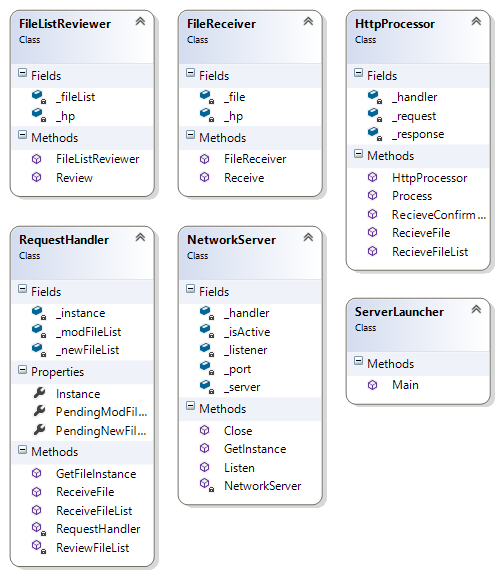
\includegraphics[width=\textwidth]{illustrations/classDiagrams/serverCD.png}
  \caption{Class Diagram Server}
  \label{classdiagramserver}
\end{figure}
\begin{figure}[H]
  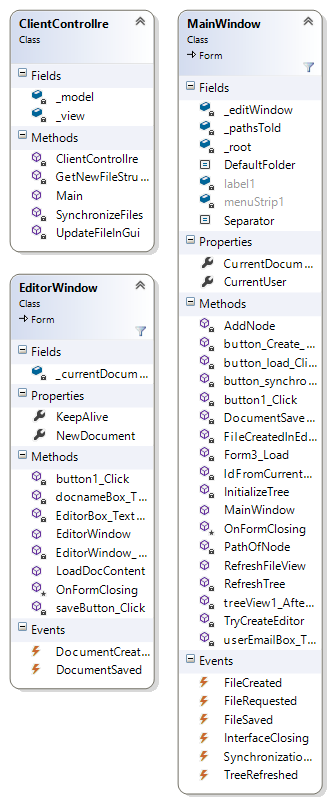
\includegraphics[width=\textwidth]{illustrations/classDiagrams/offlineCD.png}
  \caption{Class Diagram Client}
  \label{classdiagramclient}
\end{figure}
\begin{figure}[H]
  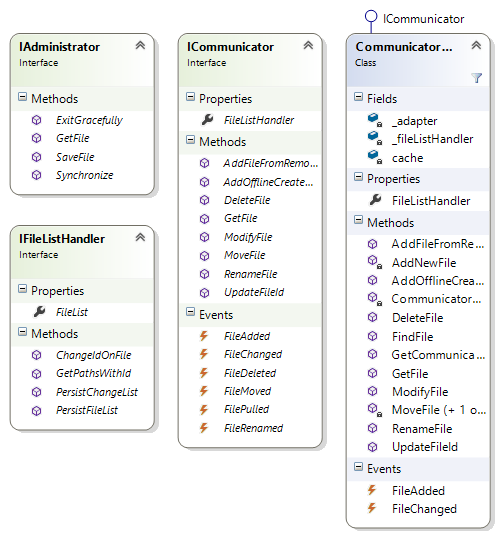
\includegraphics[width=\textwidth]{illustrations/classDiagrams/partPersistence.png}
  \caption{Class Diagram Persistence}
\end{figure}
\begin{figure}[H]
  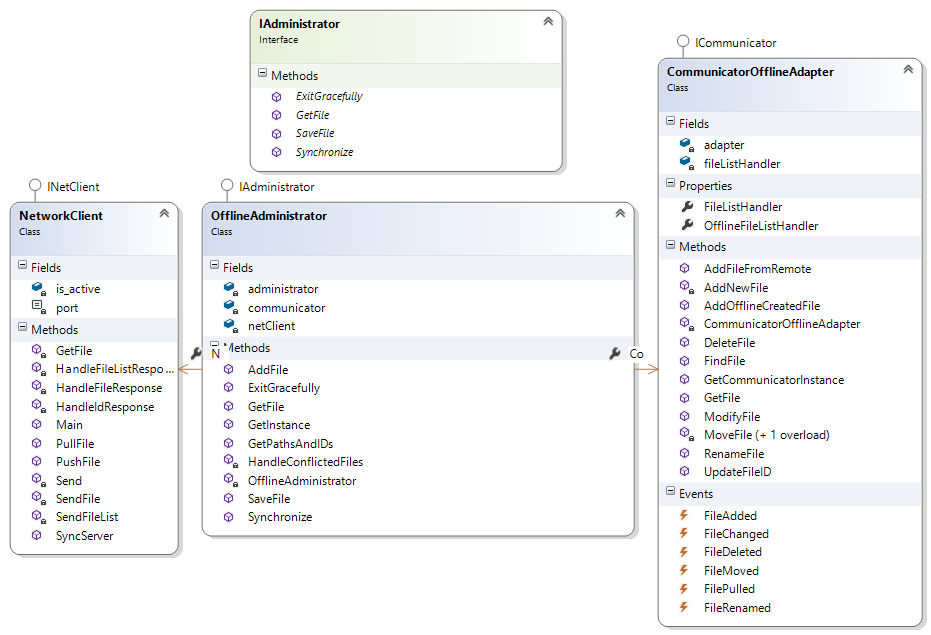
\includegraphics[width=\textwidth]{illustrations/classDiagrams/ModelFacade_CD.png}
  \caption{Class Diagram Model Facade}
\end{figure}
\begin{figure}[H]
  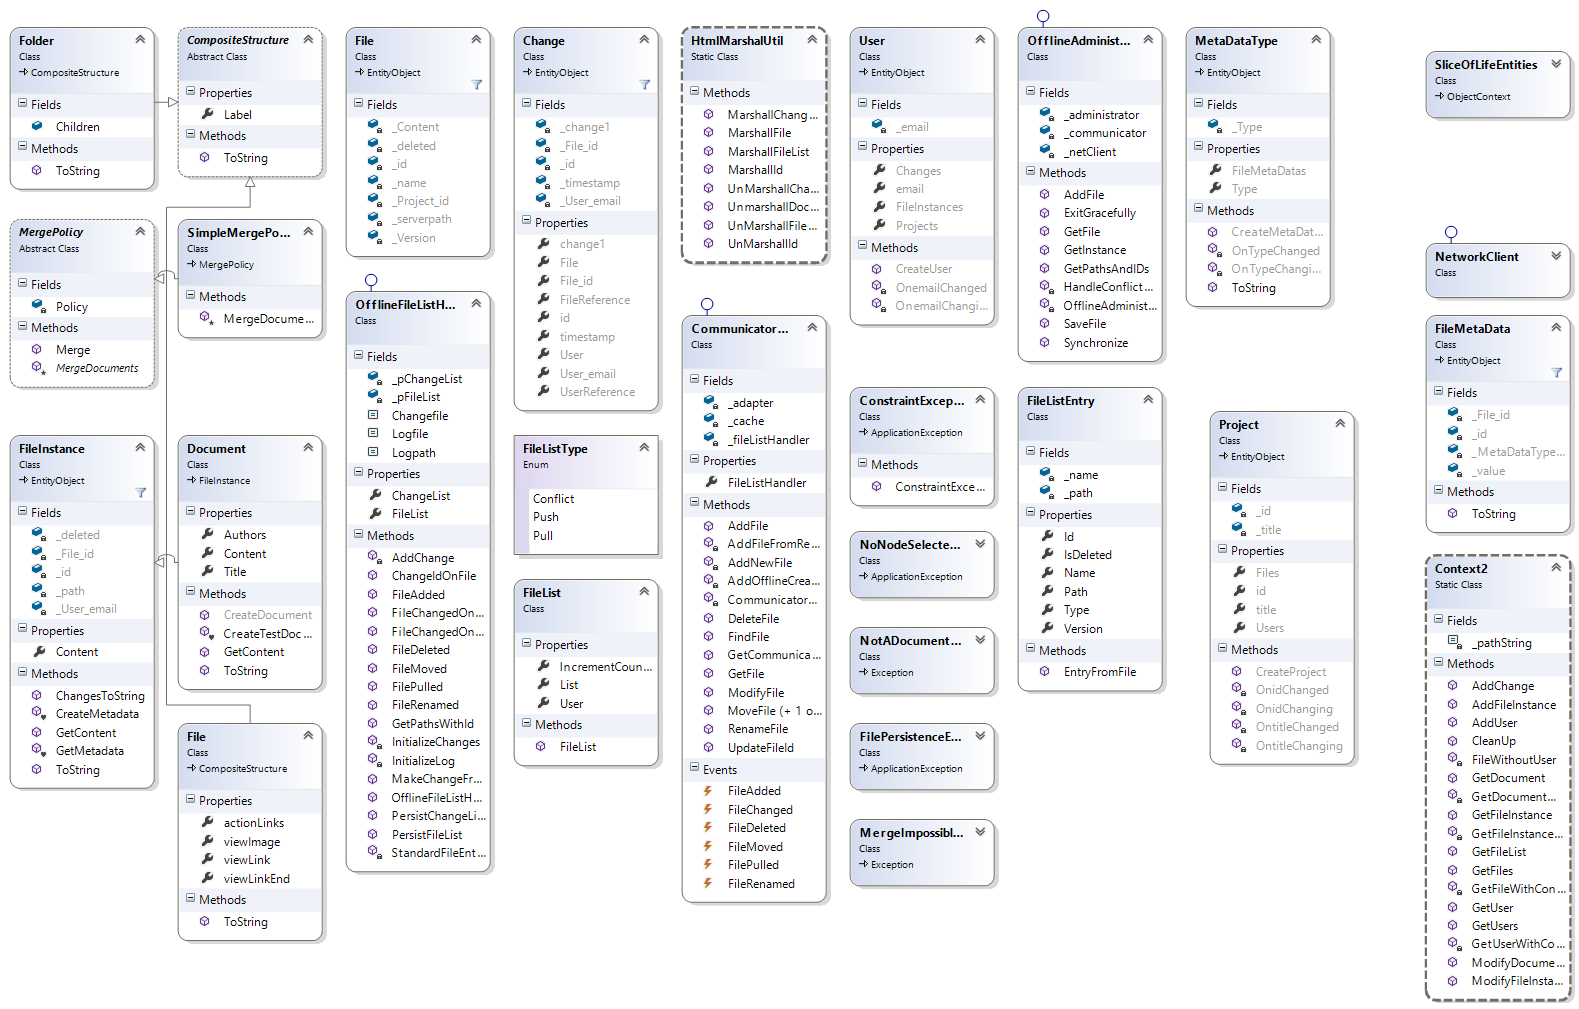
\includegraphics[width=\textwidth]{illustrations/classDiagrams/FullModel.png}
  \caption{Class Diagram Full Model}
\end{figure}
\subsection{E-R}
\begin{figure}[H]
  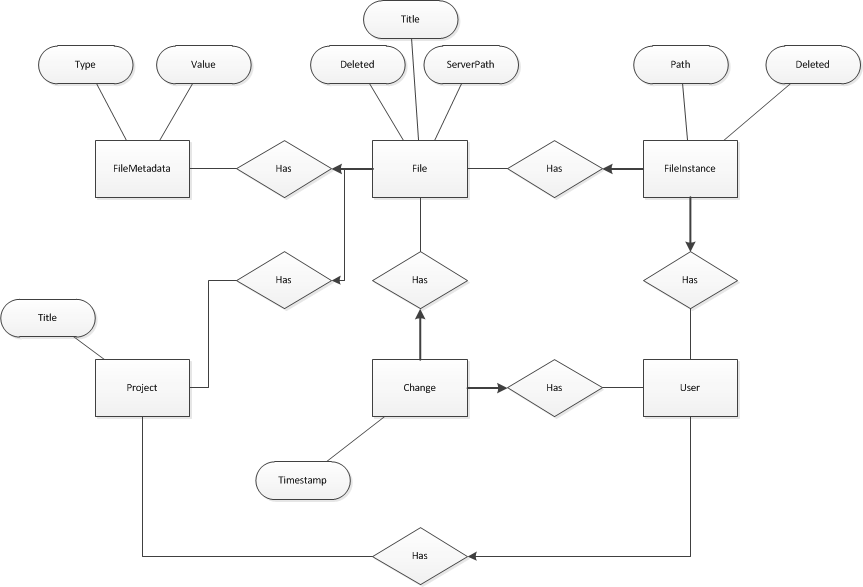
\includegraphics[width=\textwidth]{illustrations/E-R.png}
  \caption{E-R Diagram}
  \label{erdiagram}
\end{figure}
\subsection{Sequence Diagrams}
\label{sequencediagrams}
\begin{figure}[H]
  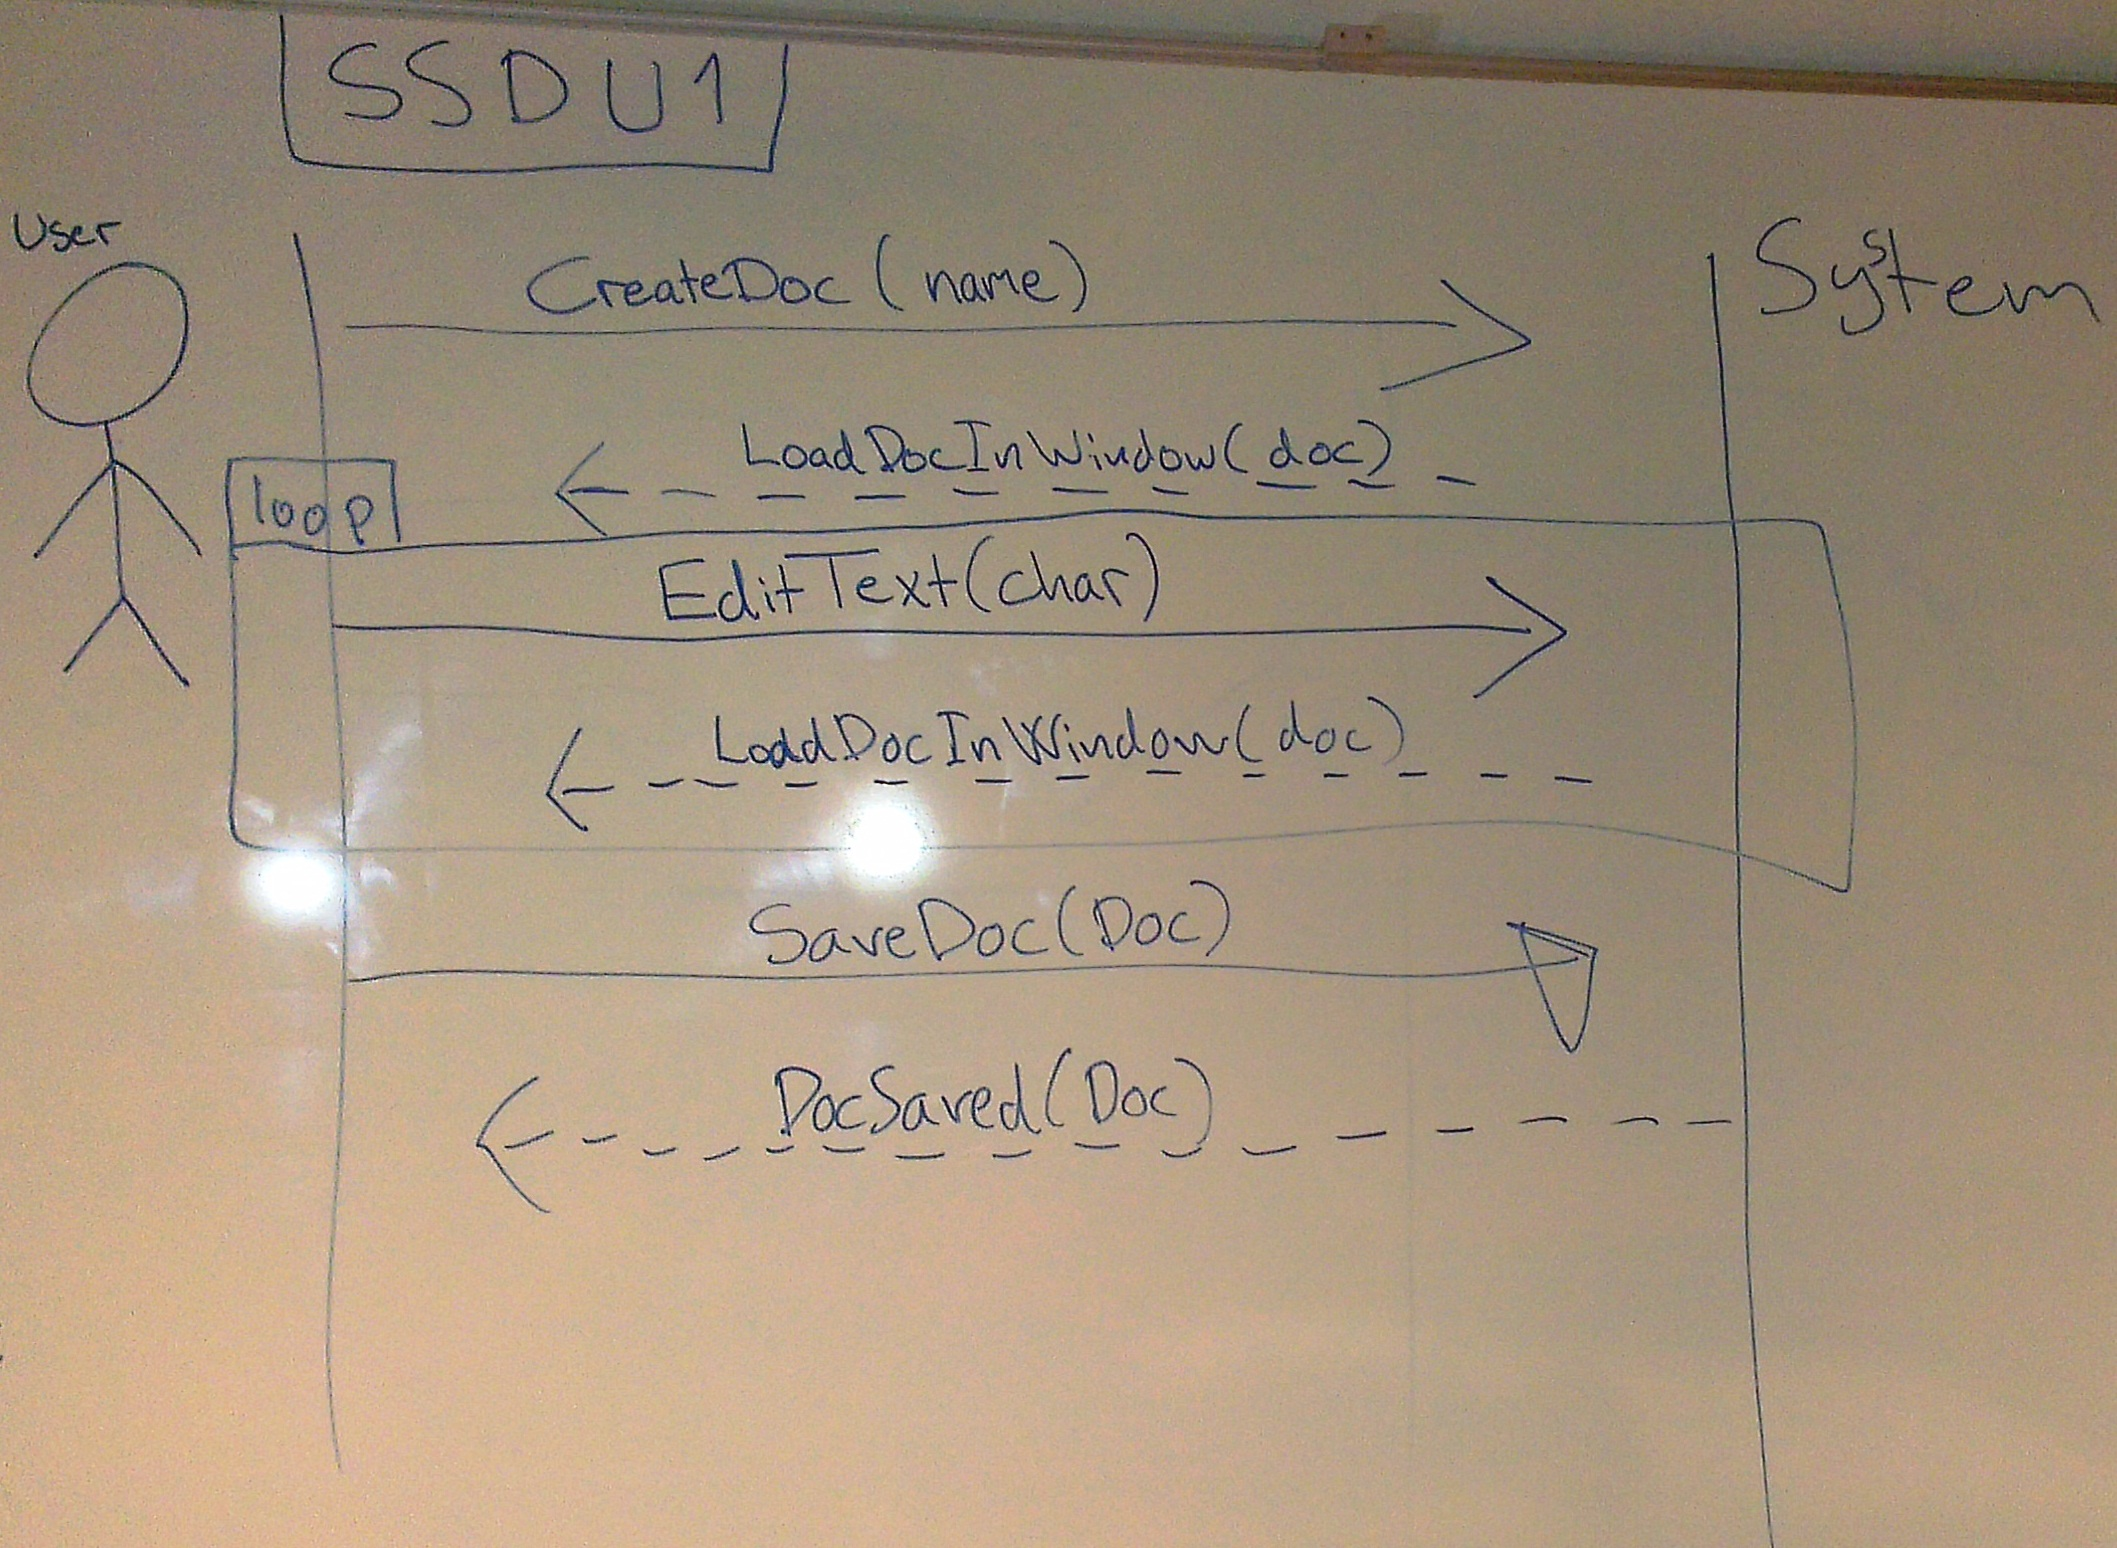
\includegraphics[width=\textwidth]{illustrations/SystemStateDiagram.jpg}
  \caption{System Sequence Diagram}
  \label{systemsequencediagram}
\end{figure}
\begin{figure}[H]
  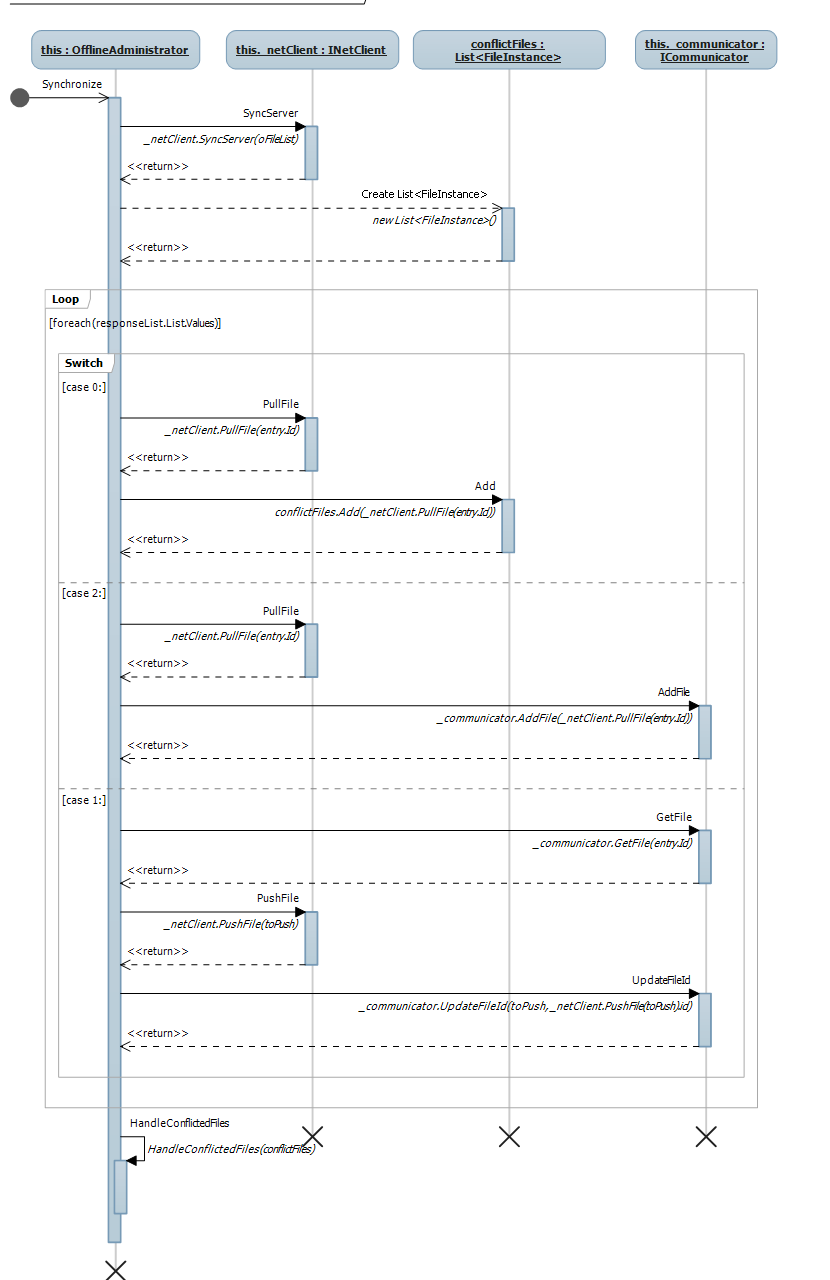
\includegraphics[width=\textwidth]{illustrations/ClientSynchfulldiagram.png}
  \caption{Server Synchronization Sequence Diagram}
  \label{serversyncsequencediagram}
\end{figure}
\begin{figure}[H]
  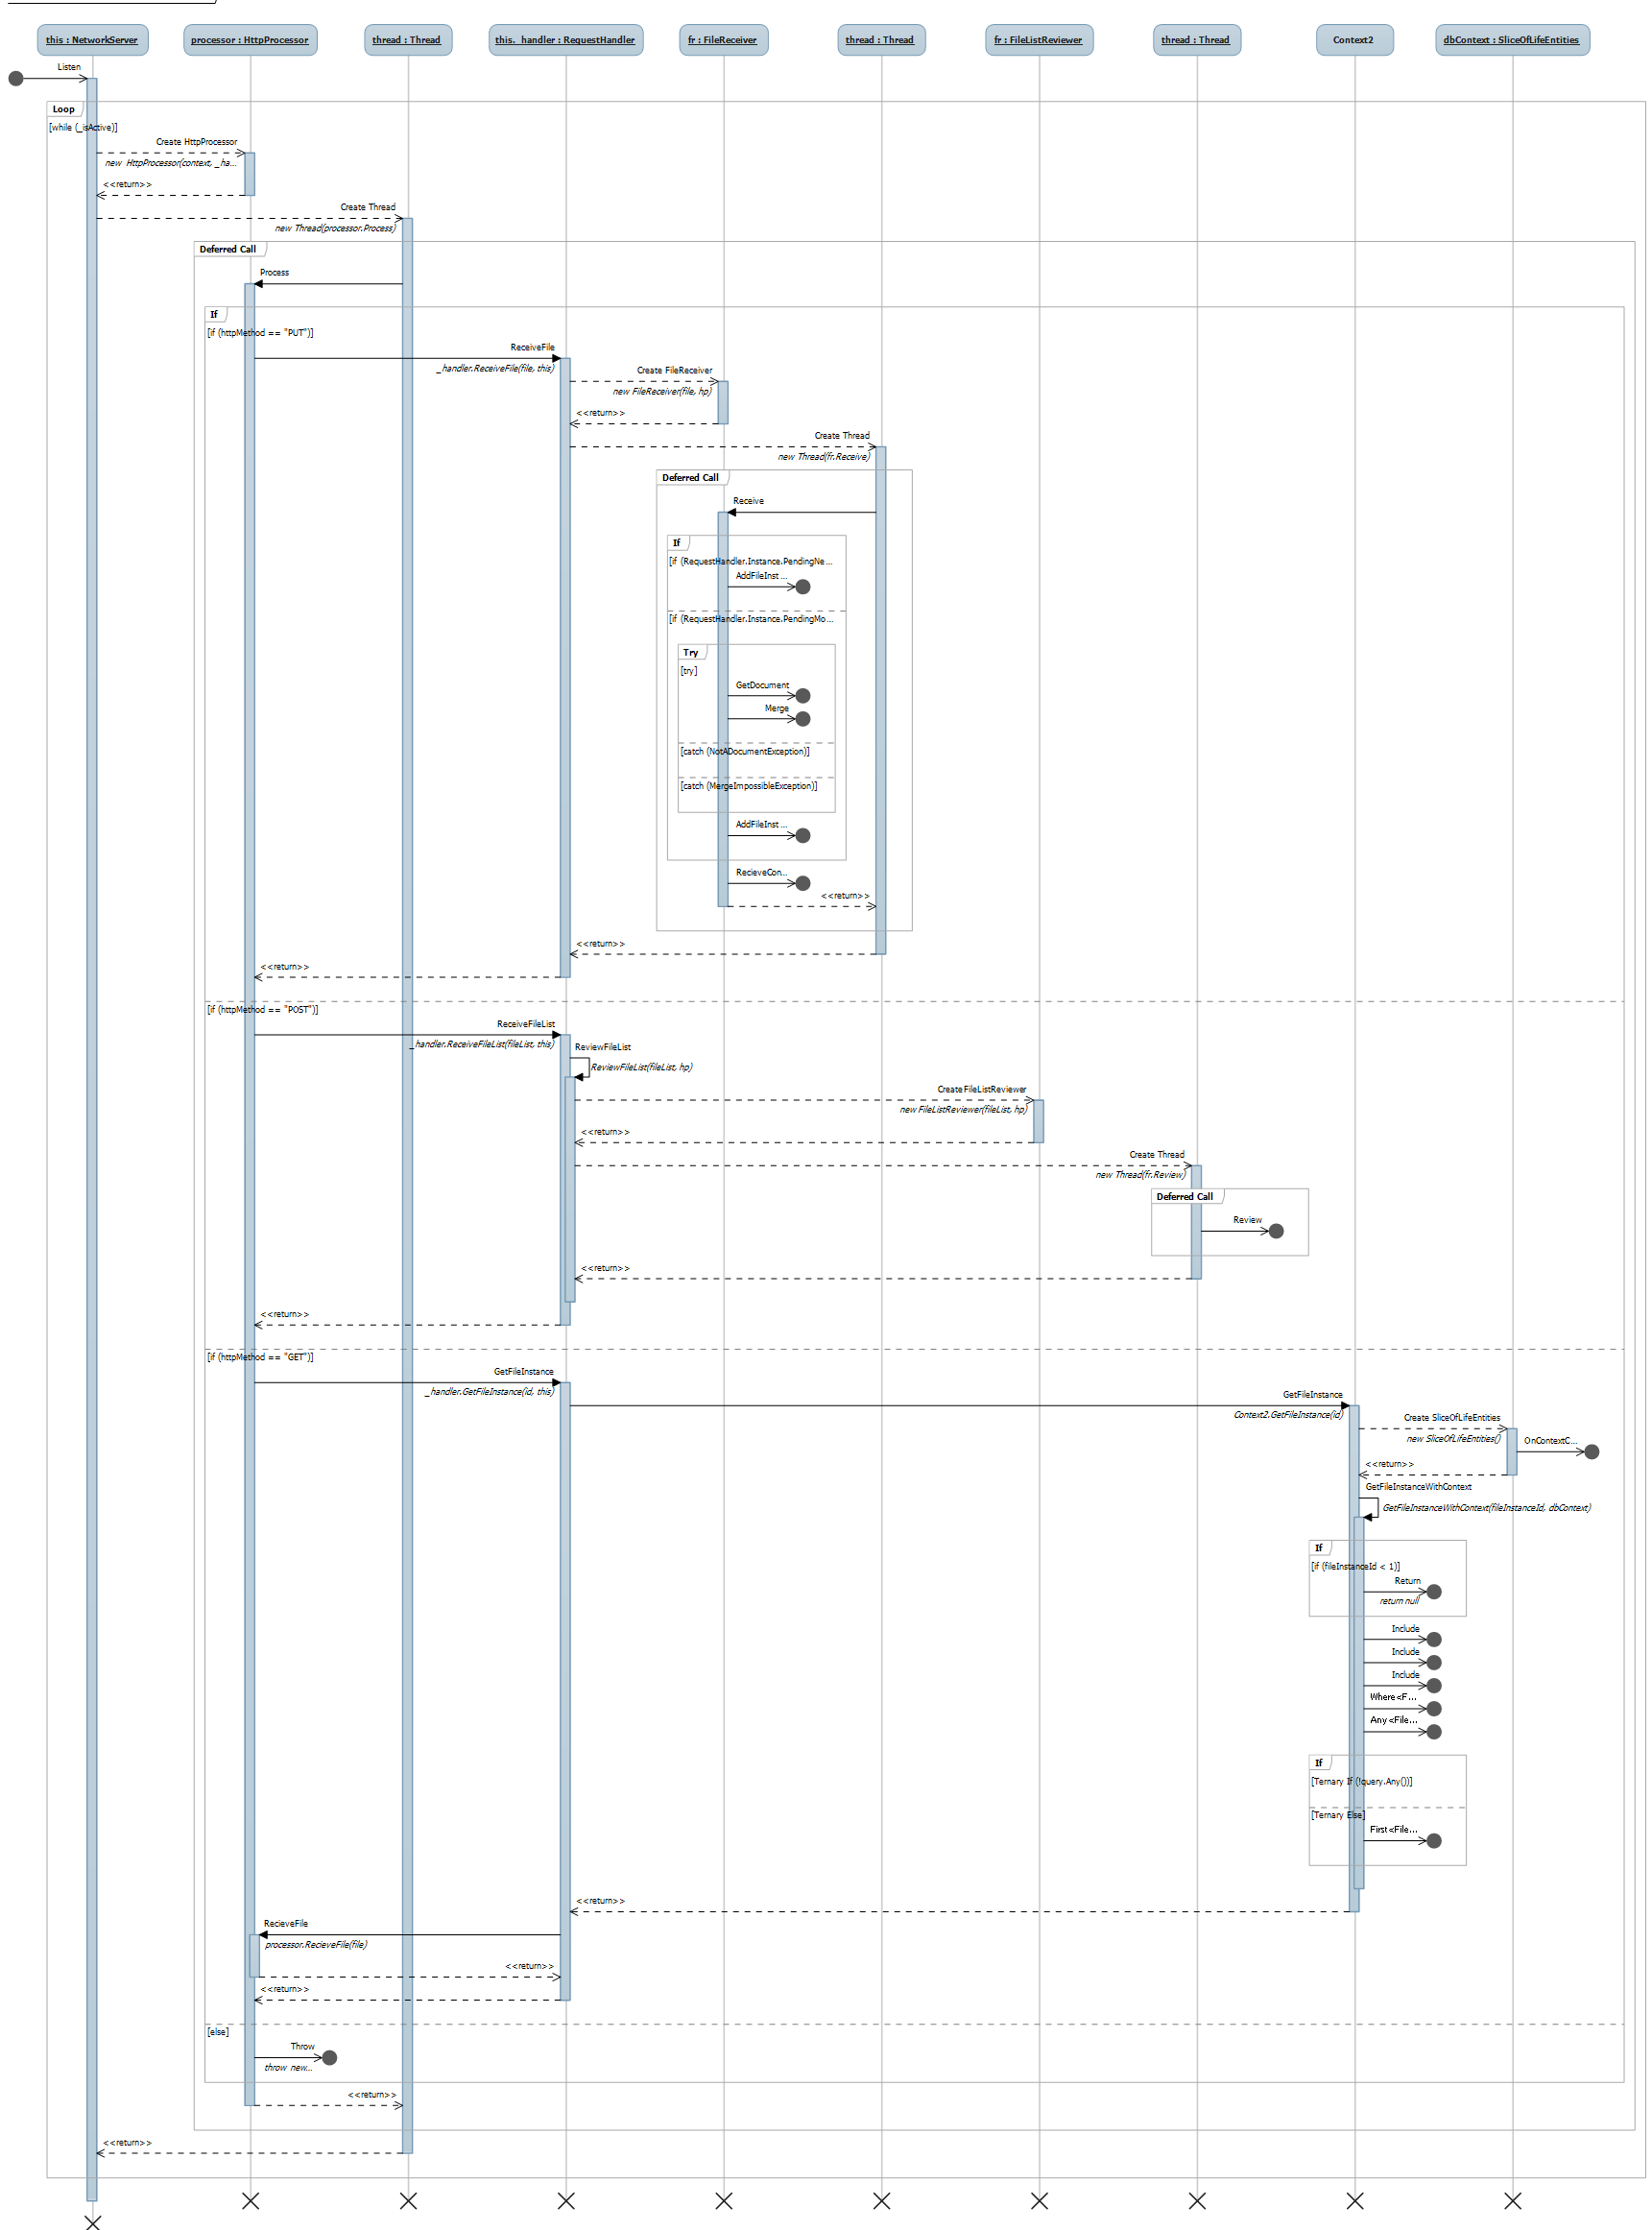
\includegraphics[width=\textwidth]{illustrations/ServerSynchfulldiagram.png}
  \caption{Client Synchronization Sequence Diagram}
  \label{clientsyncsequencediagram}
\end{figure}
\subsection{Communication Diagrams}
\begin{figure}[H]
  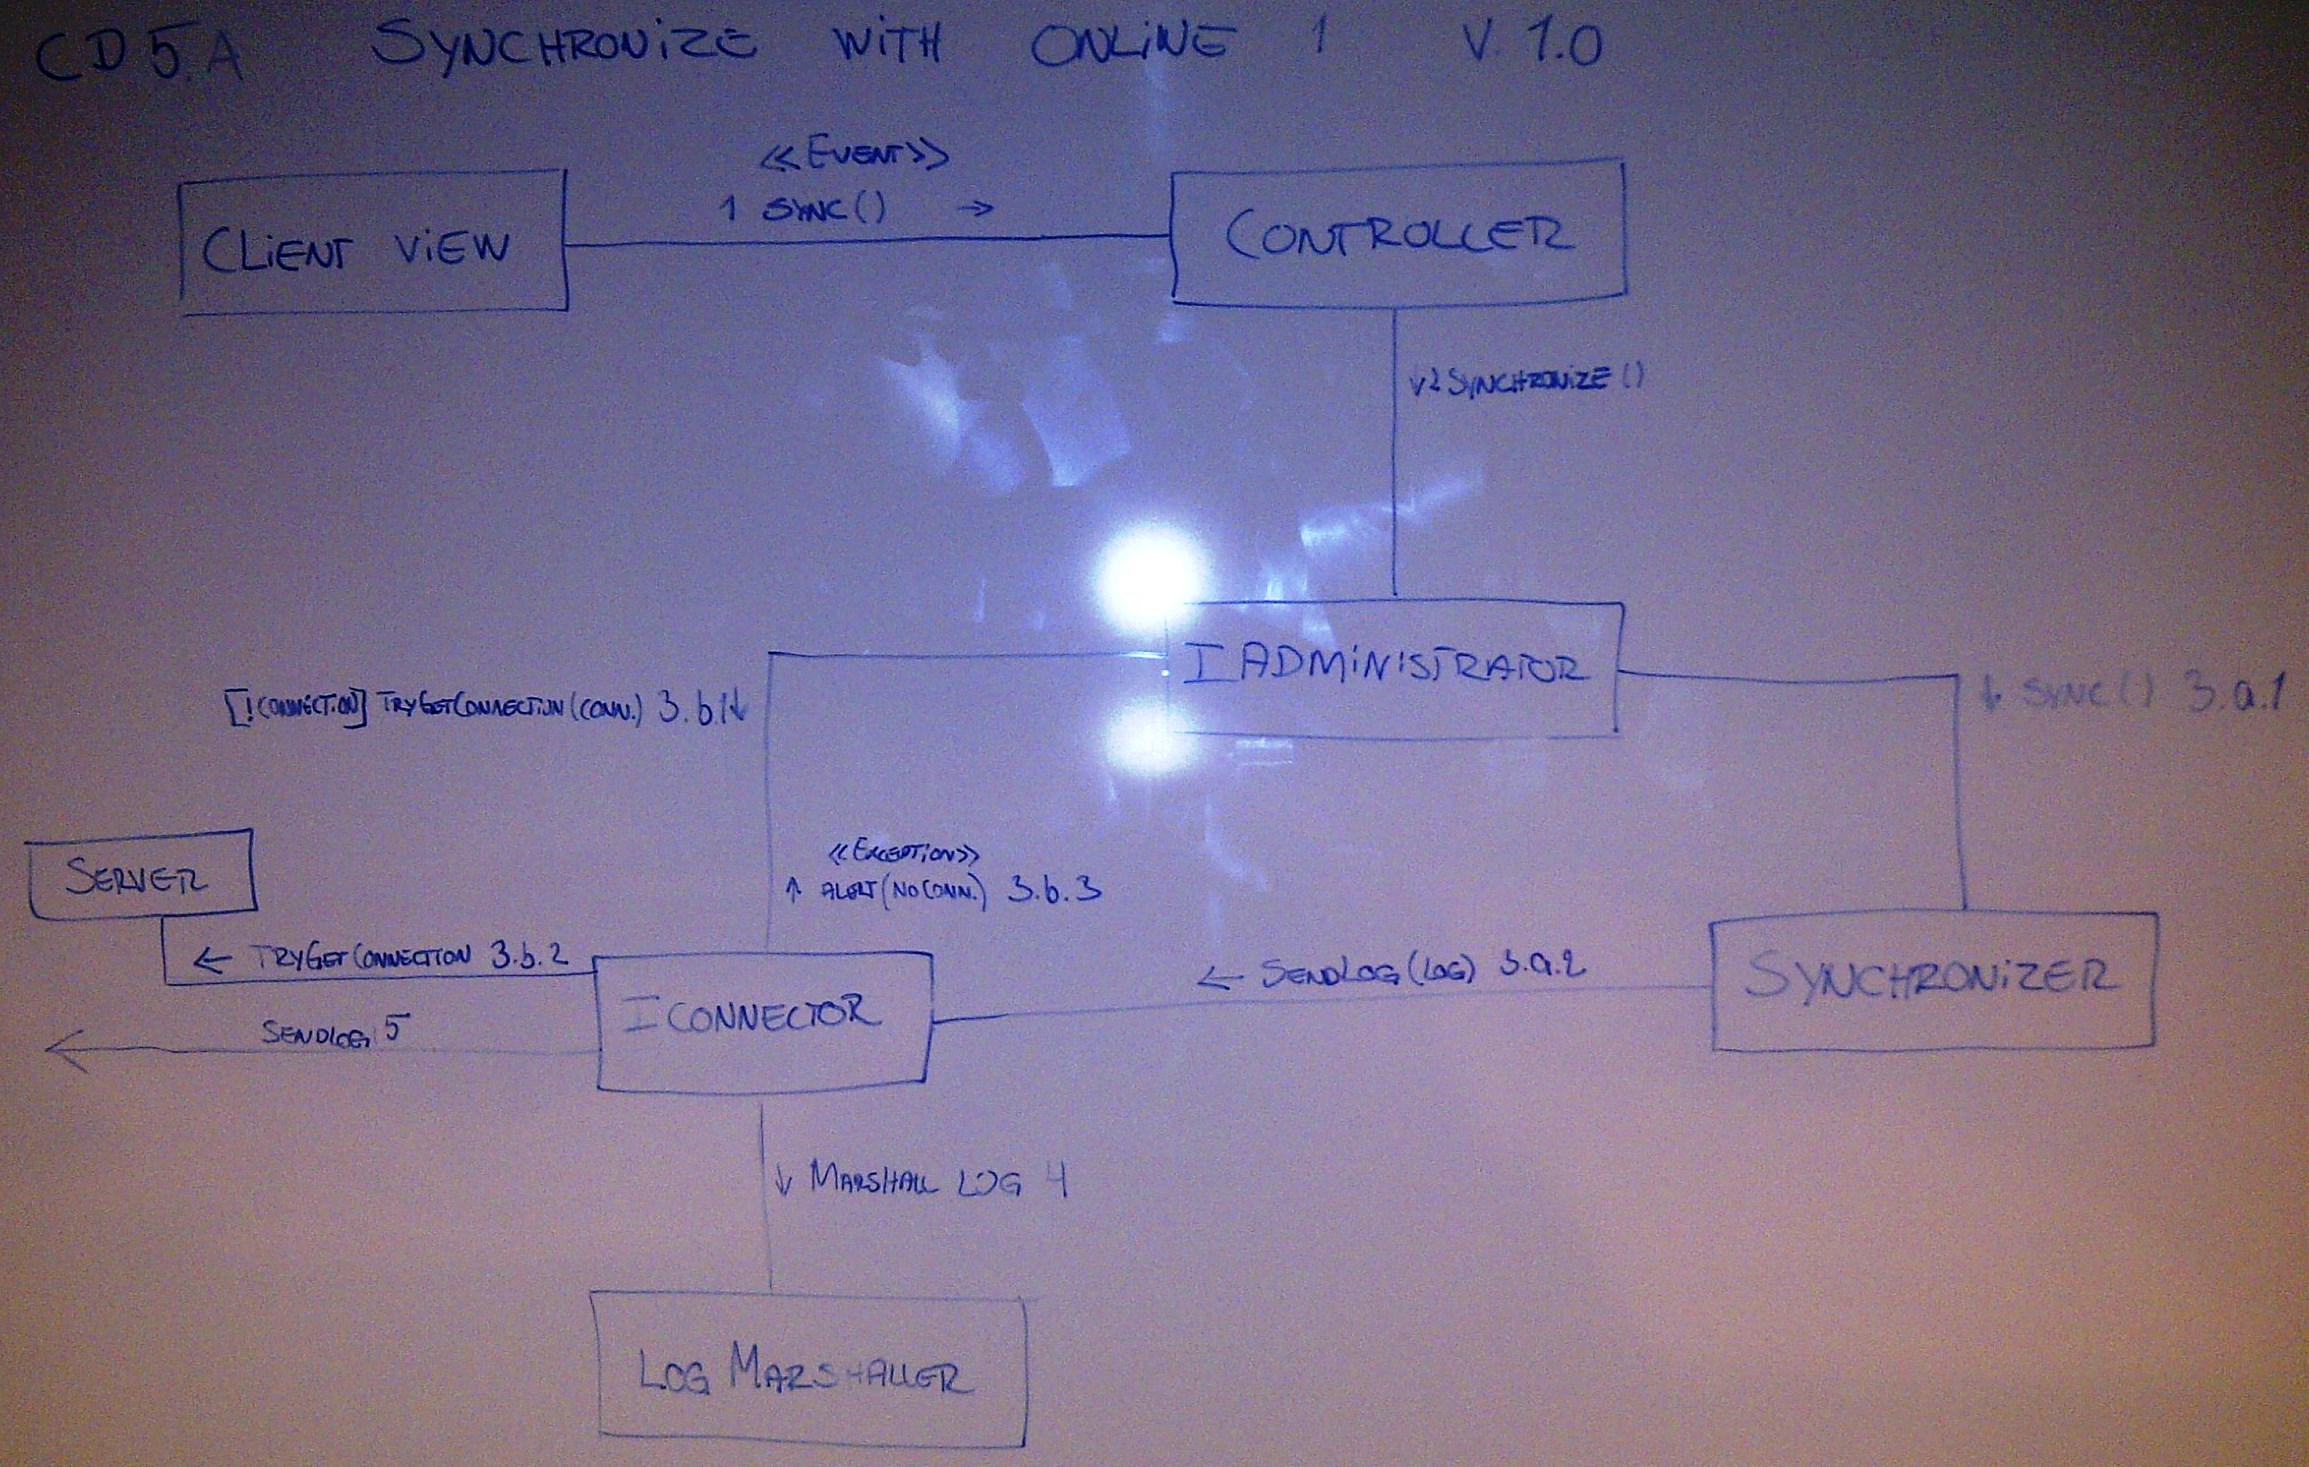
\includegraphics[width=\textwidth]{illustrations/CD5A.jpg}
  \caption{CD 5A}
  \label{CD5A}
\end{figure}
\begin{figure}[H]
  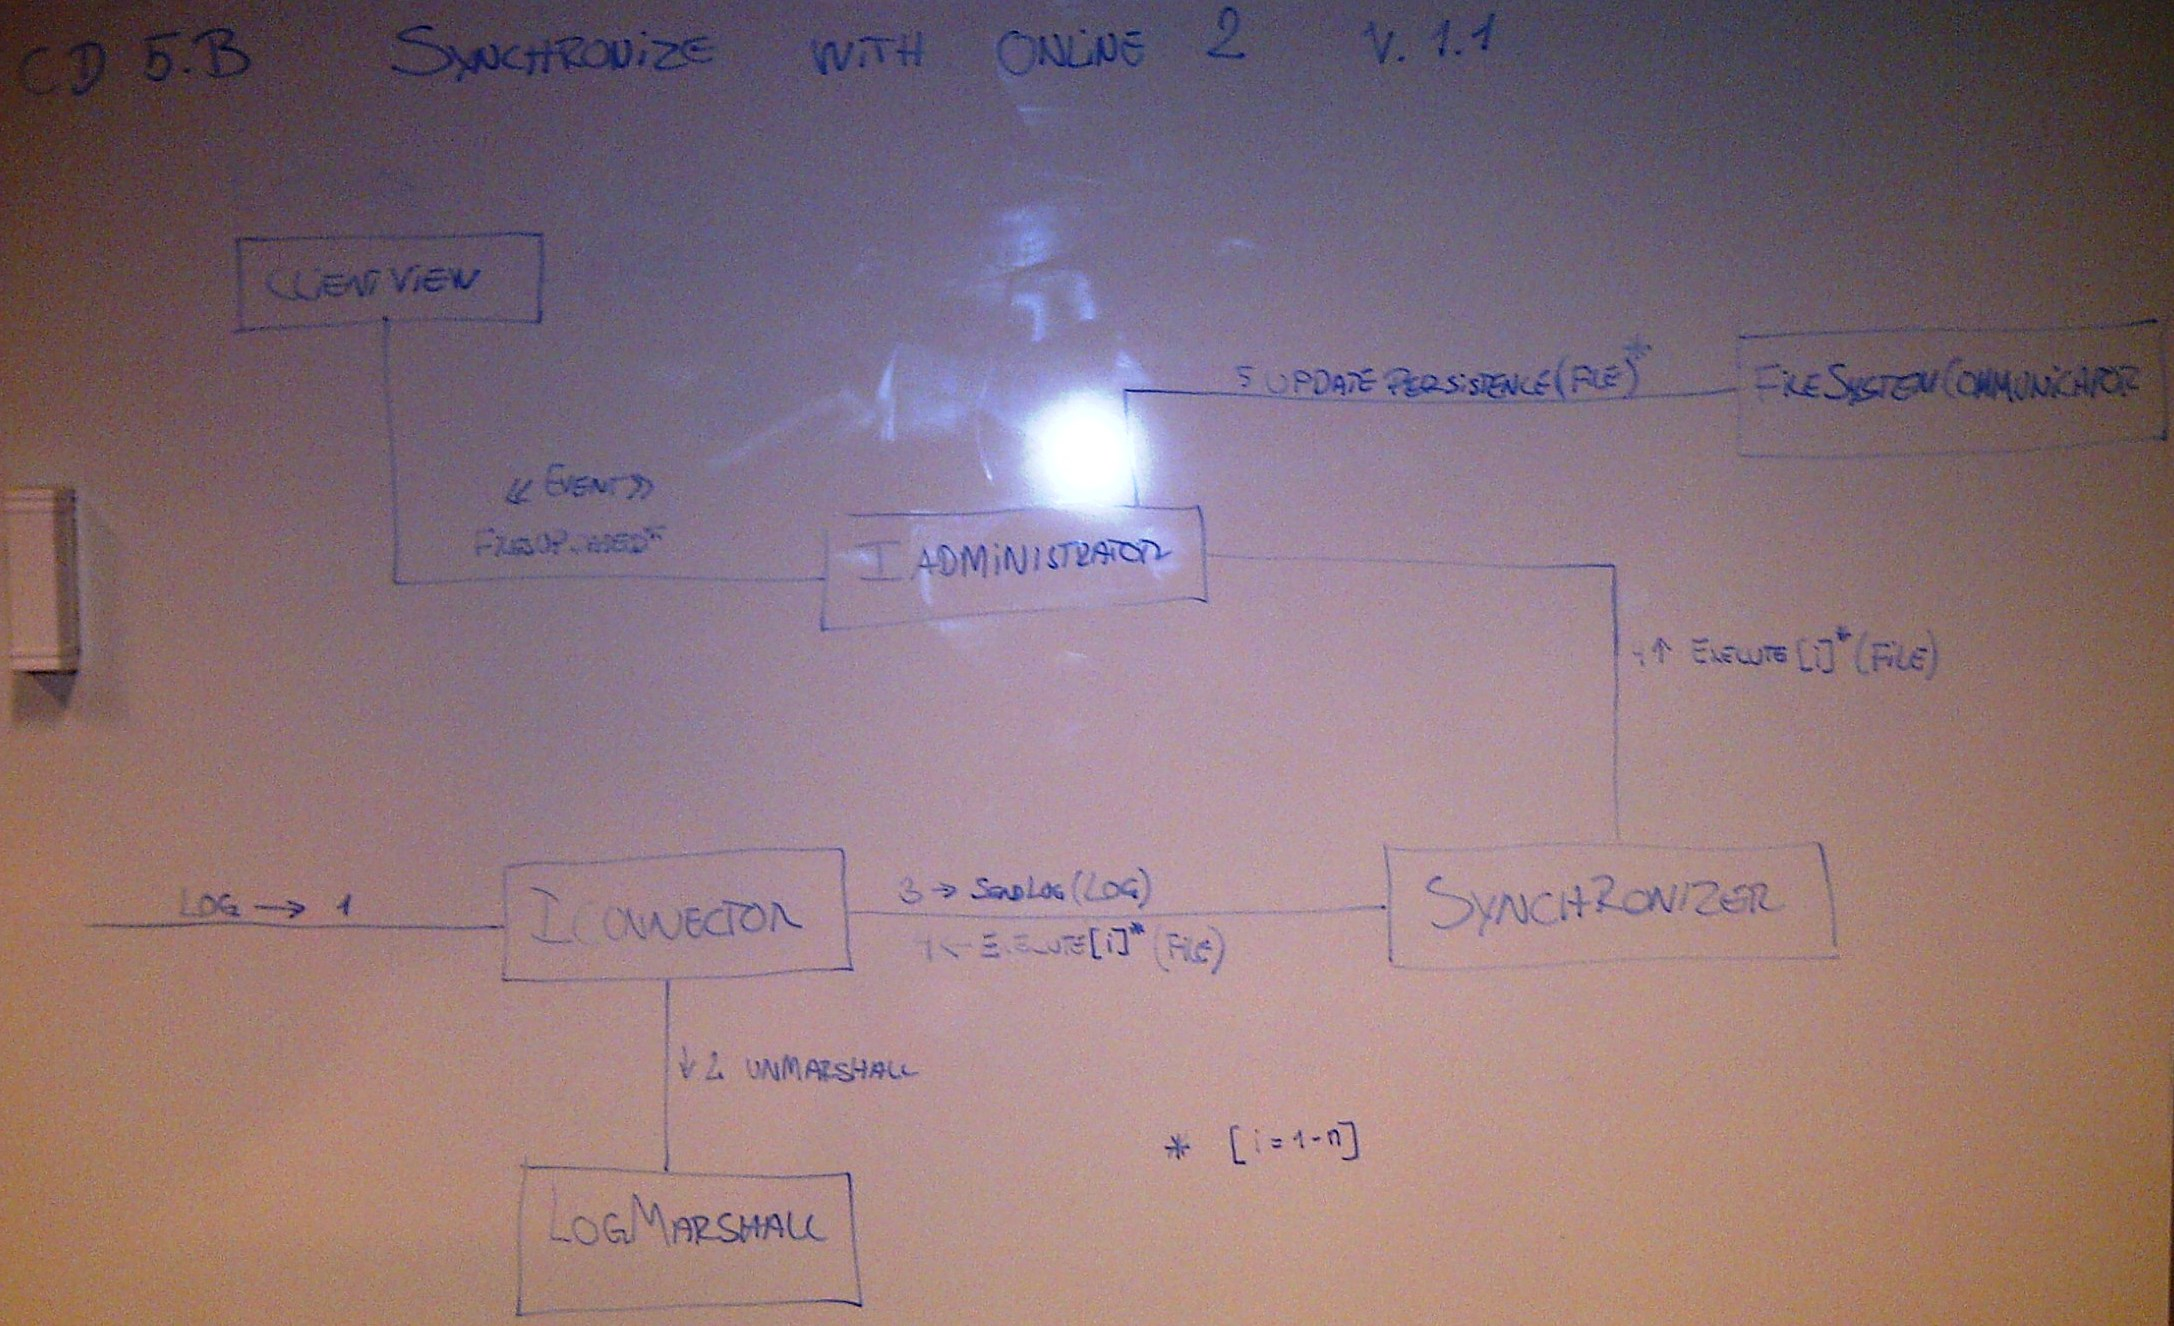
\includegraphics[width=\textwidth]{illustrations/CD5B.jpg}
  \caption{CD 5B}
  \label{CD5B}
\end{figure}
\begin{figure}[H]
  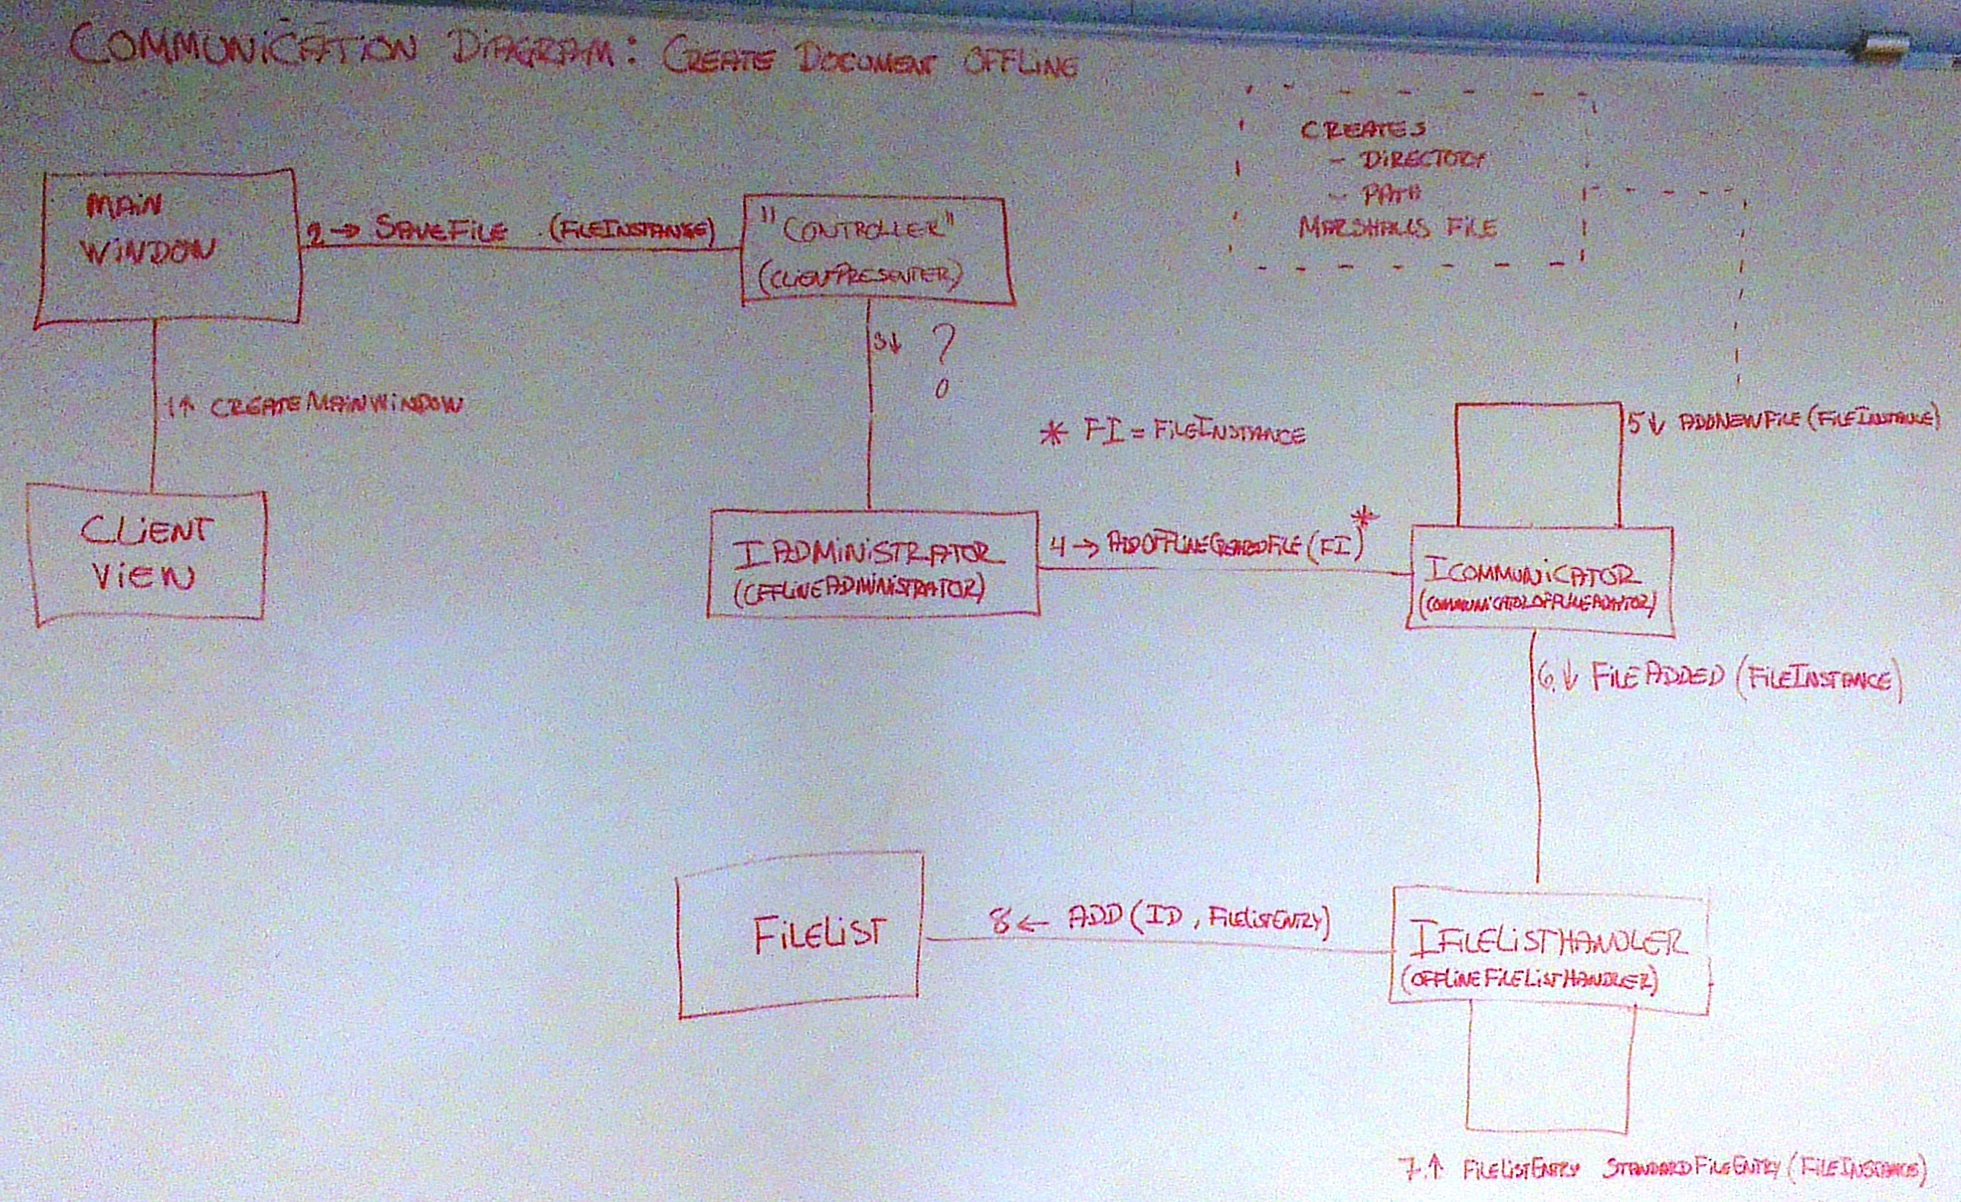
\includegraphics[width=\textwidth]{illustrations/CreateDocDiagram.jpg}
  \caption{Create Document Offline Communication Diagram}
\end{figure}
\begin{figure}[H]
  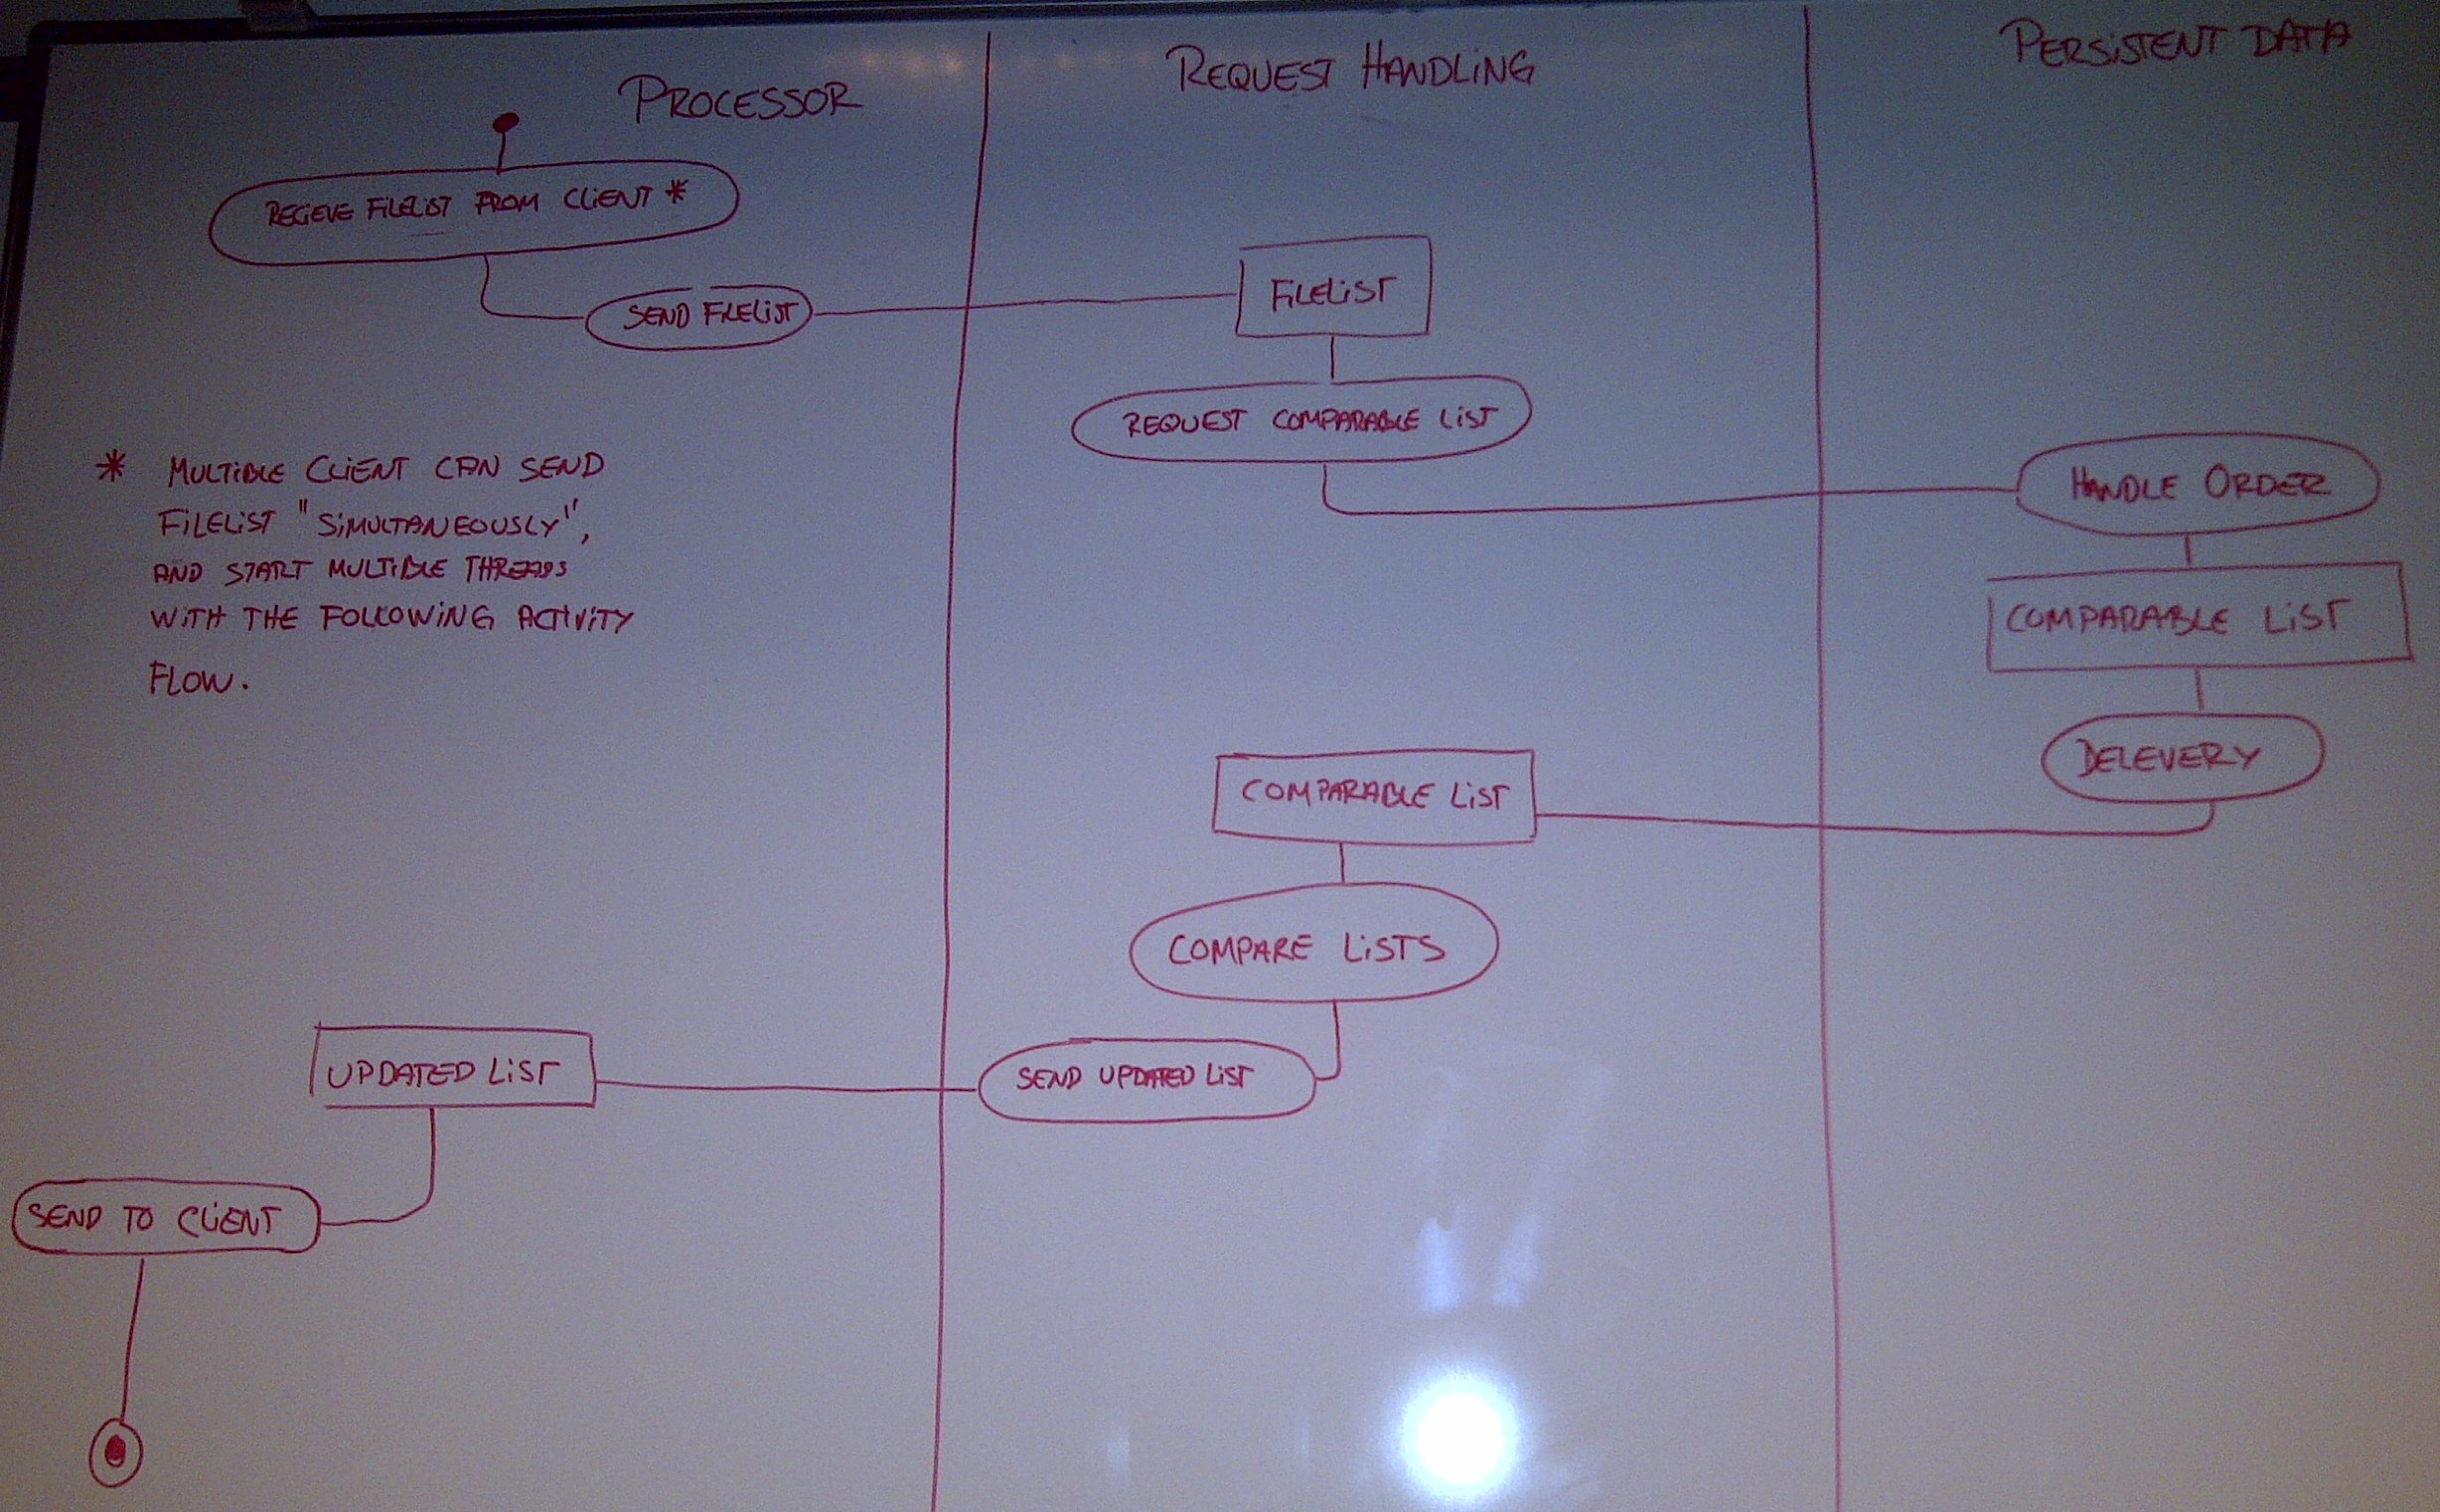
\includegraphics[width=\textwidth,natwidth=2456,natheight=1522]{illustrations/ActivityDiagram.jpg}
  \caption{Activity Diagram}
  \label{activitydiagram}
\end{figure}
%That's all folks!
\newpage